% !TeX program = xelatex
% 在本目录编译：latexmk -xelatex -outdir=../build/midterm midterm_report.tex
% 封面、正文版式和奇偶页眉沿用 main_templete.tex 与 CjC.cls。
\RequirePackage{fix-cm}
\documentclass[10.5pt,compsoc,UTF8]{CjC}
\usepackage{xeCJK}
\setCJKmainfont[Language=Chinese Simplified,BoldFont={NotoSerifCJKsc-Bold}]{NotoSerifCJKsc-Regular}
\setCJKsansfont[Language=Chinese Simplified,BoldFont={NotoSansCJKsc-Bold}]{NotoSansCJKsc-Regular}
\setCJKmonofont[Language=Chinese Simplified]{NotoSansCJKsc-Regular}
\usepackage{amsmath,amssymb}
\usepackage{booktabs,tabularx,array}
\usepackage{fancyhdr}
\usepackage[section]{placeins}
\usepackage[numbers,super,sort&compress]{natbib}
\usepackage{xurl}
\usepackage[hidelinks,bookmarksnumbered,hypertexnames=false]{hyperref}

\newcommand{\heiti}{\sffamily\bfseries}
\newcommand{\reporttitle}{面向LLM量化的多精度硬件架构设计与算力配比优化}
\fancypagestyle{midterm}{%
  \fancyhf{}
  \fancyhead[LO,RE]{\zihao{5-}\reporttitle}
  \fancyhead[LE,RO]{\zihao{5-}\thepage}
  \renewcommand{\headrulewidth}{0.5pt}
}
\DeclareRobustCommand{\midtermcontentsheading}{\zihao{3}\heiti\centerline{目\quad 录}}
\renewcommand{\contentsname}{\texorpdfstring{\midtermcontentsheading}{目录}}
\renewcommand{\figurename}{图}
\renewcommand{\tablename}{表}
\captiondelim{\quad}
\captionnamefont{\zihao{5-}}
\captiontitlefont{\zihao{5-}}
\graphicspath{{../figures/zh/}{../figures/}}
\hypersetup{pdftitle={面向LLM量化的多精度硬件架构设计与算力配比优化},pdfauthor={宋晓有}}
\setcounter{tocdepth}{2}
\renewcommand{\bibfont}{\zihao{5-}}
\setlength{\bibsep}{0pt}
\setlength{\parindent}{2em}
\setlength{\emergencystretch}{2em}
\newcolumntype{Y}{>{\raggedright\arraybackslash}X}
\newcommand{\ratio}[3]{\ensuremath{#1\!:\!#2\!:\!#3}}
\newcommand{\tabnote}[1]{\par\smallskip\begin{minipage}{\linewidth}\zihao{5-}#1\end{minipage}}

\begin{document}
\special{pdf:minorversion 7}
\hypersetup{pageanchor=false}
\begin{titlepage}
  \begin{center}
    \vspace{2cm}
    {\zihao{2}\bfseries 面向LLM量化的多精度硬件架构设计\par 与算力配比优化\par}
    \vspace{1.5cm}
    {\zihao{3}\heiti 清华大学工程硕博士培养改革专项工程硕士生\par 学位论文中期报告\par}
    \vspace{4cm}
    {\zihao{4}
    \renewcommand{\arraystretch}{1.2}
    \begin{tabular}{lc}
      \makebox[4cm][l]{研究生姓名}： & \makebox[7cm][c]{宋晓有} \\ \cline{2-2}
      \makebox[4cm][l]{学号}： & \makebox[7cm][c]{2024211104} \\ \cline{2-2}
      \makebox[4cm][l]{院系}： & \makebox[7cm][c]{集成电路学院} \\ \cline{2-2}
      \makebox[4cm][l]{专业}： & \makebox[7cm][c]{电子信息} \\ \cline{2-2}
      \makebox[4cm][l]{联合培养单位}： & \makebox[7cm][c]{华为技术有限公司} \\ \cline{2-2}
      \makebox[4cm][l]{领域}： & \makebox[7cm][c]{计算机体系结构} \\ \cline{2-2}
      \makebox[4cm][l]{学校指导教师}： & \makebox[7cm][c]{何虎} \\ \cline{2-2}
      \makebox[4cm][l]{企业指导教师}： & \makebox[7cm][c]{张帼玮} \\ \cline{2-2}
    \end{tabular}\par}
    \vfill
    {\zihao{4}二〇二六年\quad 十一月\par}
  \end{center}
\end{titlepage}

\hypersetup{pageanchor=true}
\onecolumn
\pagestyle{midterm}
\raggedbottom
\thispagestyle{empty}
\zihao{5-}
\vspace*{-13mm}
\noindent 宋晓有 \hfill 《\reporttitle》\hfill 2026 年 11 月\par
\noindent\rule[0.25\baselineskip]{\textwidth}{1pt}
\tableofcontents
\clearpage
\setcounter{page}{1}

\section*{摘\quad 要}
NVIDIA、AMD 和华为的张量计算产品采用了不同的低精度峰值算力配比。本文研究怎样用多精度点积单元实现这些配比，以及在什么负载和预算下值得增配低精度算力。在 Qwen3-4B、8B 和 14B 上完成 BF16 对照及八种权重与激活伪量化评测，NVFP4 与 MXFP4 的权重载荷接近，前者的困惑度增幅为 2.10\%--3.17\%，后者为 12.54\%--24.59\%。面向上述格式差异，提出 DP-Puzzle 点积单元，用共享乘法、对齐与归约通路保留高精度功能，通过专用计算组扩展低精度吞吐。九种 $K$ 维扩展配比均完成 11 种编码模式的数值和流水验证。在 12\,nm、1\,GHz 下，FP4 吞吐翻倍的 \ratio{1}{2}{8} 较基线增加 33.60\% 单元面积，采用共享 Q/E 组同时翻倍 FP8 与 FP4 吞吐的 \ratio{1}{4}{8} 增加 68.21\%。同构阵列可增加每个输出位置的归约长度，异构阵列也可增设专用输出列以实现同样的配比。基于已测 DP 的组合估算表明，两种方式的计算单元成本接近。前者需要更宽的 A 侧供数，后者更依赖 C/D 累加带宽。现阶段以同构 $K$ 扩展为对象，在基准面积和阵列功耗预算下按请求长度加权评估 DeepSeek-V4.1-Flash。\ratio{1}{4}{8} 的五场景综合理想 GEMM 计算加速比为 $1.145\times$。下一阶段将在昇腾 NPU 模型中对照评估两种扩展的数据搬运、存储和调度成本。

\smallskip
\noindent{\heiti 关键词}\quad 大模型量化，点积单元，混合精度，算力配比，阵列数据流

\section{选题背景及意义}

\subsection{工业界张量算力配比的演进}

张量加速器在推出 FP8、FP4 等新格式后，还要决定每种格式能够获得多少计算资源。以 BF16 为基准，若固定每拍承载的有效操作数位宽，16 位、8 位和 4 位元素的供数能力自然形成 \ratio{1}{2}{4}。在乘法阵列按窄位宽拆分、累加通路能消化更多乘积的条件下，这个输入比例可以转化为峰值计算比例。工业产品已经给出了不同的选择。表~\ref{tab:industry-ratios} 统一以单设备的稠密矩阵算力比较相应位宽档，昇腾 960PR 的路线图信息单列说明。

\begin{table}[htbp]
\centering
\caption{代表性工业产品的单设备稠密矩阵峰值与配比}
\label{tab:industry-ratios}
\begin{tabular*}{0.88\linewidth}{@{\extracolsep{\fill}}llrrrc@{}}
\toprule
厂商 & 产品 & BF16 & FP8 档 & FP4 档 & 相对 BF16 配比 \\
\midrule
NVIDIA & B200 SXM\cite{nvidiahgx} & 2.250 & 4.500 & 9.000 & \ratio{1}{2}{4} \\
       & B300 SXM\cite{nvidiahgx} & 2.250 & 4.500 & 13.500 & \ratio{1}{2}{6} \\
       & Rubin GPU\cite{nvidiaverarubin} & 4.000 & 17.500 & 35.000 & \ratio{1}{4.375}{8.75} \\
AMD & MI355X\cite{amdmi355x} & 2.517 & 5.033 & 10.066 & \ratio{1}{2}{4} \\
    & MI455X\cite{amdmi455x} & 5.033 & 20.133 & 40.265 & \ratio{1}{4}{8} \\
华为 & 昇腾 950PR（32 Cube 核）\cite{huawei950} & 0.432 & 0.865 & 1.730 & \ratio{1}{2}{4} \\
\bottomrule
\end{tabular*}
\tabnote{峰值单位为 PFLOP/s。AMD 的低精度两列取 OCP MXFP8/MXFP4，昇腾 950PR 取白皮书表 3-1 的 Cube 独立峰值。NVIDIA 两列取产品公布的对应张量精度，Rubin 的 FP4 取 NVFP4 训练档稠密值。B200 与 B300 按 HGX 八卡配置折算，BF16 和 FP8 由披露的结构化稀疏峰值换算为稠密峰值。}
\end{table}

NVIDIA B200 与 B300 的 BF16、FP8 峰值相同，B300 将稠密 FP4 峰值提高 50\%，把比例从 \ratio{1}{2}{4} 改为 \ratio{1}{2}{6}。AMD 则在 MI455X 上同时提高两个低精度档相对 BF16 的算力，配比由 MI355X 的 \ratio{1}{2}{4} 变为 \ratio{1}{4}{8}。Rubin 的稠密峰值体现出相近的联合增强方向。华为昇腾 950PR 的 Cube 采用约 \ratio{1}{2}{4} 的峰值关系。后续昇腾 960 路线纳入 HiF4 支持，并区分 960DT 与面向推理的 960PR\cite{huawei2025roadmap,huawei960roadmap}。在已见两种增配方向的基础上，本文将 \ratio{1}{2}{8} 作为单独翻倍 FP4 的对照点，用来观察继续提高 FP4 吞吐所需的开销。产品规格为候选配比提供了依据，本文进一步研究复用算术部件和专用组如何实现这些能力，以及实现成本如何随配比变化。

\subsection{模型对低精度算力的需求}

一颗芯片上的峰值配比通常随其数据通路在设计时确定，模型却可以随算法和部署方案改变各精度的用量。Transformer 的线性投影、前馈网络和注意力均包含大规模矩阵运算\cite{vaswani2017attention,qwen3technicalreport}。以 DeepSeek-V4.1-Flash 为例，路由专家的权重可使用 4 位表示，但原计算形态仍使用 FP8 激活，主注意力的部分矩阵乘使用 BF16，其他投影及索引器又可采用不同精度\cite{deepseekv41source}。当专家逐步采用 W4A4 或注意力迁移到 FP4 后，模型对 FP4 的计算需求才会进一步上升。权重表示变窄首先影响存储量，原生低精度计算能否提高速度还取决于激活格式和对应算子的硬件执行方式。

配比研究也因此包含两个相互联系的设计问题。第一，张量阵列以什么粒度增加低精度资源，才能在保留现有高精度功能的同时控制面积和功耗。第二，在固定芯片预算、精度需求变化的条件下，增配后的阵列究竟能供多少计算，哪一种配比适合目标负载。本文以点积单元为可综合的设计边界，先比较低精度资源的物理代价，再结合典型负载研究可用算力形成的条件。

\section{国内外研究现状}

\subsection{低精度格式与分块量化}

OCP 微缩放格式（Microscaling，MX）让 32 个元素共享 E8M0 尺度，MXFP8、MXFP6 和 MXFP4 分别使用不同的元素指数与尾数\cite{ocpmx2023,microscaling2023}。从电路看，二次幂尺度可以通过指数运算施加，组内低位元素仍要按各自格式解码。从数值看，同一组的峰值决定尺度，组内异常值可能把较小元素推入量化网格较粗的区域。NVFP4 保留 E2M1 元素编码，用 16 元素的 E4M3 块尺度和张量外层尺度调节范围\cite{nvidia2025nvfp4}。HiF4 以 64 元素为块，再分 8 元素和 4 元素小组调节微指数\cite{hifloat4}。两者能够更细地调整组内范围，也使点积单元增加了尺度尾数处理与块边界控制。

GPTQ 通过近似二阶信息补偿权重量化误差，AWQ 利用激活统计保护敏感权重\cite{gptq,awq}。RaZeR 研究 NVFP4 的转换误差及额外编码点的利用\cite{razer}。这些方法都可以改变同一格式的模型表现。为确定格式自身的表达代价，本文在 Qwen3 上先固定直接舍入与计算流程，分别观察权重和激活重建、端到端模型评分与紧密存储容量。该设置可回答某个格式在相同实验条件下付出了多少精度代价，为选取硬件支持的格式提供依据。

\subsection{多精度乘法与移位对齐的复用}

多精度点积由乘积生成、指数对齐及多项规约组成，各部分的复用条件不同。乘法器产生的部分积彼此独立，适合根据目标精度决定怎样拼接或分发。Bit Fusion 将窄位乘法单元通过移位加法组合成较宽运算\cite{bitfusion2018}。Park 等在统一数据通路上让 FP16 尾数乘法与 INT8/INT4 点积复用乘积和归约资源\cite{park2022unified}。TransDot 则在同一硬件上选择性重组部分积，支持标量、高低精度分区和点积累加\cite{transdot2026}。这些方法都利用了高精度模式需要宽乘积、低精度模式需要更多独立窄乘积的差异。本文可由同一乘法阵列拼出宽尾数，也可在窄模式下对多个元素同时相乘，保留流水的发射速率。

浮点乘积加法还要解决小数点位置不同的问题。指数比较、位移量生成和可变移位器随并行路数增加，其中移位网络的代价同时受数据宽度和最大移位量影响。Abdel-Aziz 等人的工作分析了浮点对齐与加法的成本，并以时间分解支持较高精度\cite{abdelaziz2021overheads}。TransDot 把宽桶形移位器分区，使其在宽操作与多路窄操作之间切换，分区选择需要额外门控。Ten-Four 让不同格式的点积接入共享规约后端，MXDOTP 把微缩放处理纳入点积路径并累加至 FP32\cite{tenfour,islamoglu2025mxdotp}。对本文的格式集合，T/H/Q 可共享一套局部对齐路径，E2M1 和 HiF4 的部分指数又能精确融入定点幅值。因此，可以保持统一规约后端，同时在 E 专用组中省去逐乘积的宽移位。这给出了单独扩大 FP4 算力时有机会降低成本的电路依据。

\subsection{累加项的接入与浮点结果的形成}

多路点积加累加项 $C$ 可采用不同的数据路径。将已规格化的点积作为一个 FP32 数输出，再使用独立浮点加法器计算 $C$ 的和，便于复用既有加法器。若点积已经舍入为 FP32，则 $C$ 无法恢复被第一次舍入移除的信息。另一种安排是在产生点积后保留扩展精度，延后注入 $C$，仍然可以只在末尾进行一次 FP32 舍入。Lutz 等在 FP8 四项点积中比较了延后接入和提前共同对齐两种融合方案。延后方案能够复用经改造的 FP32 加法路径，提前方案则把乘积与累加项纳入共同位权的规约网络\cite{lutz2024fused}。MiniFloat-NN 的 ExSdotp 也将两个低精度乘积与一个较宽的累加项融合\cite{bertaccini2022minifloat}。

对位宽受限的融合结构，共同窗口应覆盖组部分和与 $C$ 的动态范围。实际误差还受对齐截断、累加顺序以及接近零时的相消影响\cite{sun2023tensorcores,xie2025mmasim,tensorgauge}。本文将 $C$ 接在组完成块缩放之后、全 DP 完成规约之前。这样组内对齐只面对乘积的指数差，组间窗口才处理部分和与 FP32 $C$ 的指数差。Timeloop 和 LLMCompass 分别提供了算子映射、存储复用与大模型推理的系统评估方法\cite{timeloop2019,llmcompass}。本文先以阵列带宽充足为条件建立算力配比的比较基准，再在后续工作中将阵列供数和输出累加纳入同一评价。

\section{Qwen3 量化精度与存储代价}
\label{sec:quant}

研究从格式选择入手。对于 FP4，三种格式的标称位宽相同，权重压缩比也接近。若模型精度差异较大，硬件就需要同时支持几种缩放语义，单凭位宽决定支持对象容易忽略格式的使用条件。因而选择模型规模不同、结构相近的 Qwen3 作为对照，将操作数编码带来的数值差异与推理内核性能分开观察。

\subsection{量化方法与模型接入}

实验采用 Qwen3-4B、8B 和 14B，分别以原 BF16 推理为对照，对每种模型测试 MXFP8 E4M3/E5M2、MXFP6 E2M3/E3M2、MXINT8、MXFP4、NVFP4 和 HiF4，共 27 个配置。量化对象为各解码层的七个线性投影，即注意力的 $Q/K/V/O$ 投影和前馈网络的 gate、up、down 投影。权重在加载后沿每行归约维 $K$ 一次性转换。激活沿相同方向逐次转换，其中 $Q/K/V$ 共用一个输入转换点，gate/up 共用一个输入转换点，加上 $O$、down 投影，共四处。词嵌入、归一化、输出词表头和注意力内部 $QK^{\mathsf T}$、$PV$ 沿用原模型计算。各配置将重建值写回 BF16，在同一 BF16 Linear 上执行，从而把比较集中在操作数的取值网格、缩放与舍入差异上。

对一个有符号数据块 $x_g$，记 $a_g=\max_i |x_{g,i}|$，$q_{\max}$ 为元素的最大有限幅值。MX 浮点沿 $K$ 每 32 个元素一组，正常非零组选择覆盖 $a_g/q_{\max}$ 的最小二次幂尺度 $s_g$。转换可写成
\begin{equation}
  s_g=2^{\lceil\log_2(a_g/q_{\max})\rceil},\qquad
  q_i=\mathrm{Sat}\bigl(\mathrm{RNE}_{\mathcal{F}}(x_{g,i}/s_g)\bigr),\qquad
  \hat{x}_{g,i}=\mathrm{BF16}(s_gq_i).
\end{equation}
其中 RNE 为最近偶数舍入，$\mathcal{F}$ 为目标元素格式。程序以指数拆分取得尺度指数，处理全零组和指数边界，保留次正规格点。MXINT8 使用整数格点 $[-127,127]$，将固定的 $2^{-6}$ 因子吸收到整数步长中。其极端尺度限幅沿用实验配方，普通范围的重参数化和 OCP 规定的全范围尺度边界分别记录。NVFP4 先按权重张量或激活样本选取 FP32 外层尺度，再将每 16 个元素的块尺度舍入到 E4M3，元素按 E2M1 量化。激活外层尺度只读取本样本有效位置，填充值置零后参与峰值归约。HiF4 按 64、8 和 4 个元素计算分层峰值，得到 E6M2 基准尺度和两级微指数，再舍入 S1P2 幅值。所有配置采用同一直接舍入流程。模型按各格式固有的分组与尺度机制转换，比较结果体现这些编解码选择的综合影响。

\subsection{评测协议与实现核验}

困惑度（Perplexity，PPL）使用 WikiText-2 raw 测试集\cite{merity2016pointer}。将全文分词后切为 146 个互不重叠的 2048-token 窗口。每个窗口一次前向，位置 $t$ 的词表分布给真实的第 $t+1$ 个 token 打分。窗口第一个 token 提供上下文，末尾输出无同窗口标签，因而每个窗口计分 2047 个目标，共 $N=298862$ 个。对全部有效目标的负对数似然求平均，再取指数
\begin{equation}
  \mathrm{PPL}=\exp\left(-\frac{1}{N}\sum_{w=1}^{146}\sum_{t=1}^{2047}
    \log p_\theta(x_{w,t+1}\mid x_{w,1:t})\right).
\end{equation}
NVFP4 按完整窗口确定激活外层尺度，因此同一前缀的量化重建值可能随窗口其余内容变化。所得 PPL 对应整窗口量化的前向设置。

任务正确率采用 MMLU-Redux 2.0 的 57 学科、5700 道题\cite{mmluredux}，在固定的零样本文本模板下取最后有效位置的 A、B、C、D 候选 token logits，以最大者为预测。评分采用数据中原始 \texttt{answer} 标签。两个指标分别度量真实 token 的概率与选项判定的一致率。PPL 批大小固定为 2，选择题批大小固定为 8，按长度分批和右侧填充，同一模型下各精度使用相同题单、窗口和批次形状。

实现验证覆盖量化格点、舍入饱和、padding 隔离、投影接入、标签移位和四选一评分。27 个配置均经过真实模型的短输入冒烟检查。完整实验保留逐窗口 NLL、目标数，以及逐题 ID、四项 logits 和评分。复核共覆盖 3942 个窗口、8069274 个预测目标和 153900 条题目评分，逐配置复算 PPL、正确率及四选项最大值。另抽样检查 Qwen3-14B 第 0、20、39 层的权重和激活，使用独立转换实现比对 MX 格点，并检查模型前向的量化调用次数。

\subsection{不同格式的表达误差与模型效果}

% 表中 27 个配置取自 low_precision_quant/results/summary.tsv 与 summary_14b.tsv。
\begin{table}[htbp]
\centering
\caption{Qwen3 权重与激活量化的模型效果}
\label{tab:qwen}
\zihao{5-}
\begin{tabular}{@{}lrrrrrr@{}}
\toprule
& \multicolumn{2}{c}{Qwen3-4B} & \multicolumn{2}{c}{Qwen3-8B} & \multicolumn{2}{c}{Qwen3-14B} \\
\cmidrule(lr){2-3}\cmidrule(lr){4-5}\cmidrule(l){6-7}
格式 & PPL & 正确率（\%） & PPL & 正确率（\%） & PPL & 正确率（\%） \\
\midrule
BF16 & 13.6565 & 69.95 & 9.7249 & 73.67 & 8.6487 & 78.60 \\
MXFP8 E5M2 & 13.9816 & 68.53 & 9.8311 & 73.33 & 8.7059 & 77.26 \\
MXFP8 E4M3 & 13.8375 & 69.84 & 9.7672 & 73.58 & 8.6744 & 78.26 \\
MXFP6 E3M2 & 13.9959 & 68.49 & 9.8375 & 73.28 & 8.7138 & 77.12 \\
MXFP6 E2M3 & 13.8385 & 69.49 & 9.7547 & 73.75 & 8.6613 & 78.11 \\
MXINT8 & 13.6664 & 69.68 & 9.7305 & 74.05 & 8.6485 & 78.56 \\
MXFP4 & 17.0149 & 62.14 & 10.9446 & 67.30 & 9.8913 & 73.25 \\
NVFP4 & 13.9431 & 65.00 & 10.0136 & 72.75 & 8.9225 & 76.61 \\
HiF4 & 15.1682 & 66.51 & 10.1778 & 71.95 & 9.0221 & 76.18 \\
\bottomrule
\end{tabular}
\end{table}

表~\ref{tab:qwen} 表明，在相同 32 元素块的条件下，三个模型的 E4M3 相对 E5M2、E2M3 相对 E3M2 均获得更低 PPL 和更高正确率。以 8B 为例，MXFP6 E2M3 的 PPL 为 9.7547，接近 BF16 的 9.7249，也低于 MXFP8 E4M3 的 9.7672。E2M3 与 E4M3 同为三位显式尾数，前者靠较窄指数节省存储。能否利用这两位节省，取决于组级缩放后的指数范围能否覆盖主要数值。由表~\ref{tab:qs} 可见，E4M3 和 E2M3 对抽样激活的重建误差小于对应的两位显式尾数格式。该实验中的共享尺度已经承担一部分动态范围调整，组内增加尾数位有利于细化常见数值附近的格点。

\begin{table}[htbp]
\centering
\caption{Qwen3-14B 抽样张量的量化信噪比（dB）}
\label{tab:qs}
\zihao{5-}
\begin{tabular}{@{}lrr@{}}
\toprule
格式 & 权重 & 激活 \\
\midrule
MXINT8       & 41.36 & 39.40 \\
MXFP8 E5M2   & 25.56 & 26.34 \\
MXFP8 E4M3   & 31.51 & 30.52 \\
MXFP6 E3M2   & 25.56 & 26.31 \\
MXFP6 E2M3   & 30.87 & 29.33 \\
MXFP4        & 18.52 & 19.25 \\
\bottomrule
\end{tabular}
\tabnote{采用 $-10\log_{10}[\sum_i(\hat{x}_i-x_i)^2/\sum_i x_i^2]$，数值越大表示重建误差越小。抽样包含 9240576 个权重元素和 1572864 个激活元素。}
\end{table}

在 4 位组内，NVFP4 在三个模型上的 PPL 均最低。4B 的选择题正确率以 HiF4 最高（66.51\%），8B 和 14B 则以 NVFP4 最高（72.75\% 和 76.61\%）。与 BF16 相比，MXFP4 在三种模型上的正确率分别下降 7.81、6.37 和 5.35 个百分点。NVFP4 和 HiF4 都引入了比 MXFP4 更细的尺度调节，这两种格式在本次评测中均取得较低 PPL 和较高正确率。PPL 与正确率给出的组内排序有时不同。MXINT8 的 PPL 接近 BF16，14B 的净答对数仅少 2 题，其中 31 题由对转错，29 题由错转对。这个例子体现了汇总正确率与逐题预测变化的区别。

\subsection{权重量化的存储成本}

按紧密打包计算，$b$ 位元素每 $g$ 项共享 $s$ 位元数据时，块内平均开销为 $b+s/g$ bit/权重。NVFP4 另需每个权重矩阵一个 FP32 外层尺度。表~\ref{tab:storage} 同时给出可量化权重的相对降幅，以及 Qwen3-14B 的权重载荷估计。该模型每层有七个投影，共 40 层，合计约 132.12 亿个投影权重，占原 BF16 参数载荷的 89.46\%。按原记录中的 29.5366 GB BF16 张量载荷，保持其余参数不变，替换上述矩阵的权重与尺度编码。表中 GB 按 $10^9$ 字节计，文件头、对齐填充、激活及 KV 缓存另计。MXFP6 的 6.25 bit 对应压缩存储，送入当前 DP 接口时按 8 位槽展开。

\begin{table}[htbp]
\centering
\caption{紧密打包下的权重载荷估计}
\label{tab:storage}
\zihao{5-}
\begin{tabular}{@{}lrrrr@{}}
\toprule
格式 & 平均 bit/权重 & 可量化部分节省（\%） & 14B 载荷（GB） & 整体节省（\%） \\
\midrule
BF16           & 16.00 & 0     & 29.54 & 0 \\
MXFP8/MXINT8   &  8.25 & 48.44 & 16.74 & 43.33 \\
MXFP6          &  6.25 & 60.94 & 13.43 & 54.52 \\
MXFP4          &  4.25 & 73.44 & 10.13 & 65.70 \\
NVFP4          &  4.50 & 71.88 & 10.54 & 64.30 \\
HiF4           &  4.50 & 71.88 & 10.54 & 64.30 \\
\bottomrule
\end{tabular}
\tabnote{NVFP4 的 4.50 bit 为块内开销，整模型估算已另计 280 个 FP32 外层尺度。HiF4 的 64 元素块包含 8 位基准尺度及 24 位微指数。}
\end{table}

在该例中，MXFP6 E2M3 相对 MXFP8 进一步节省约 3.30 GB 参数载荷，14B 的 PPL 从 8.6744（MXFP8 E4M3）变为 8.6613，正确率下降约 0.16 个百分点。NVFP4 相较 MXFP4 多约 0.41 GB 权重载荷，但 14B 的 PPL 从 9.8913 降到 8.9225。这样的差异说明，压缩率与可接受的精度损失须按格式联合评估。该存储分析按编码推算，本阶段的软件伪量化以 BF16 容器保存重建值。

\section{可组合多精度点积单元的设计与验证}
\label{sec:dp}

面向上述配比，完整复制高精度 DP 会同时增加各档算力，配比本身不变。DP-Puzzle 将能复用的乘法、指数对齐和归约固定在基线组内，将需要独立扩展的低精度通路封装为专用组。组是连接格式意义与硬件开销的关键边界。同一尺度范围内可以先局部求和再施加尺度，跨不同范围则把部分和统一成可供后端比较和对齐的表示。

\subsection{运算定义与组粒度选择}

一个 DP 请求计算同一输出坐标上的点积加数，即
\begin{equation}
  D=\mathcal{R}\left(C+\sum_{i=0}^{K-1}\mathcal{D}_A(a_i)\mathcal{D}_B(b_i)\right).
  \label{eq:dot}
\end{equation}
$\mathcal{D}_A$、$\mathcal{D}_B$ 由各自编码和尺度元数据确定。浮点模式接收 FP32 的 $C$，输出 FP32 的 $D$，末级使用 RNE。式~\eqref{eq:dot} 表示数学目标，实际流水还包含有限窗口对齐。INT8 模式使用有符号二补码输入与 INT32 的 $C$，结果按模 $2^{32}$ 回绕。硬件 INT8 执行整数点积，模型实验中的 MXINT8 则把整数网格与块尺度一起用于量化和重建。NVFP4 的 DP 接口接收 16 元素块的 E4M3 尺度，张量外层尺度由上层处理。

\begin{figure}[htbp]
\centering
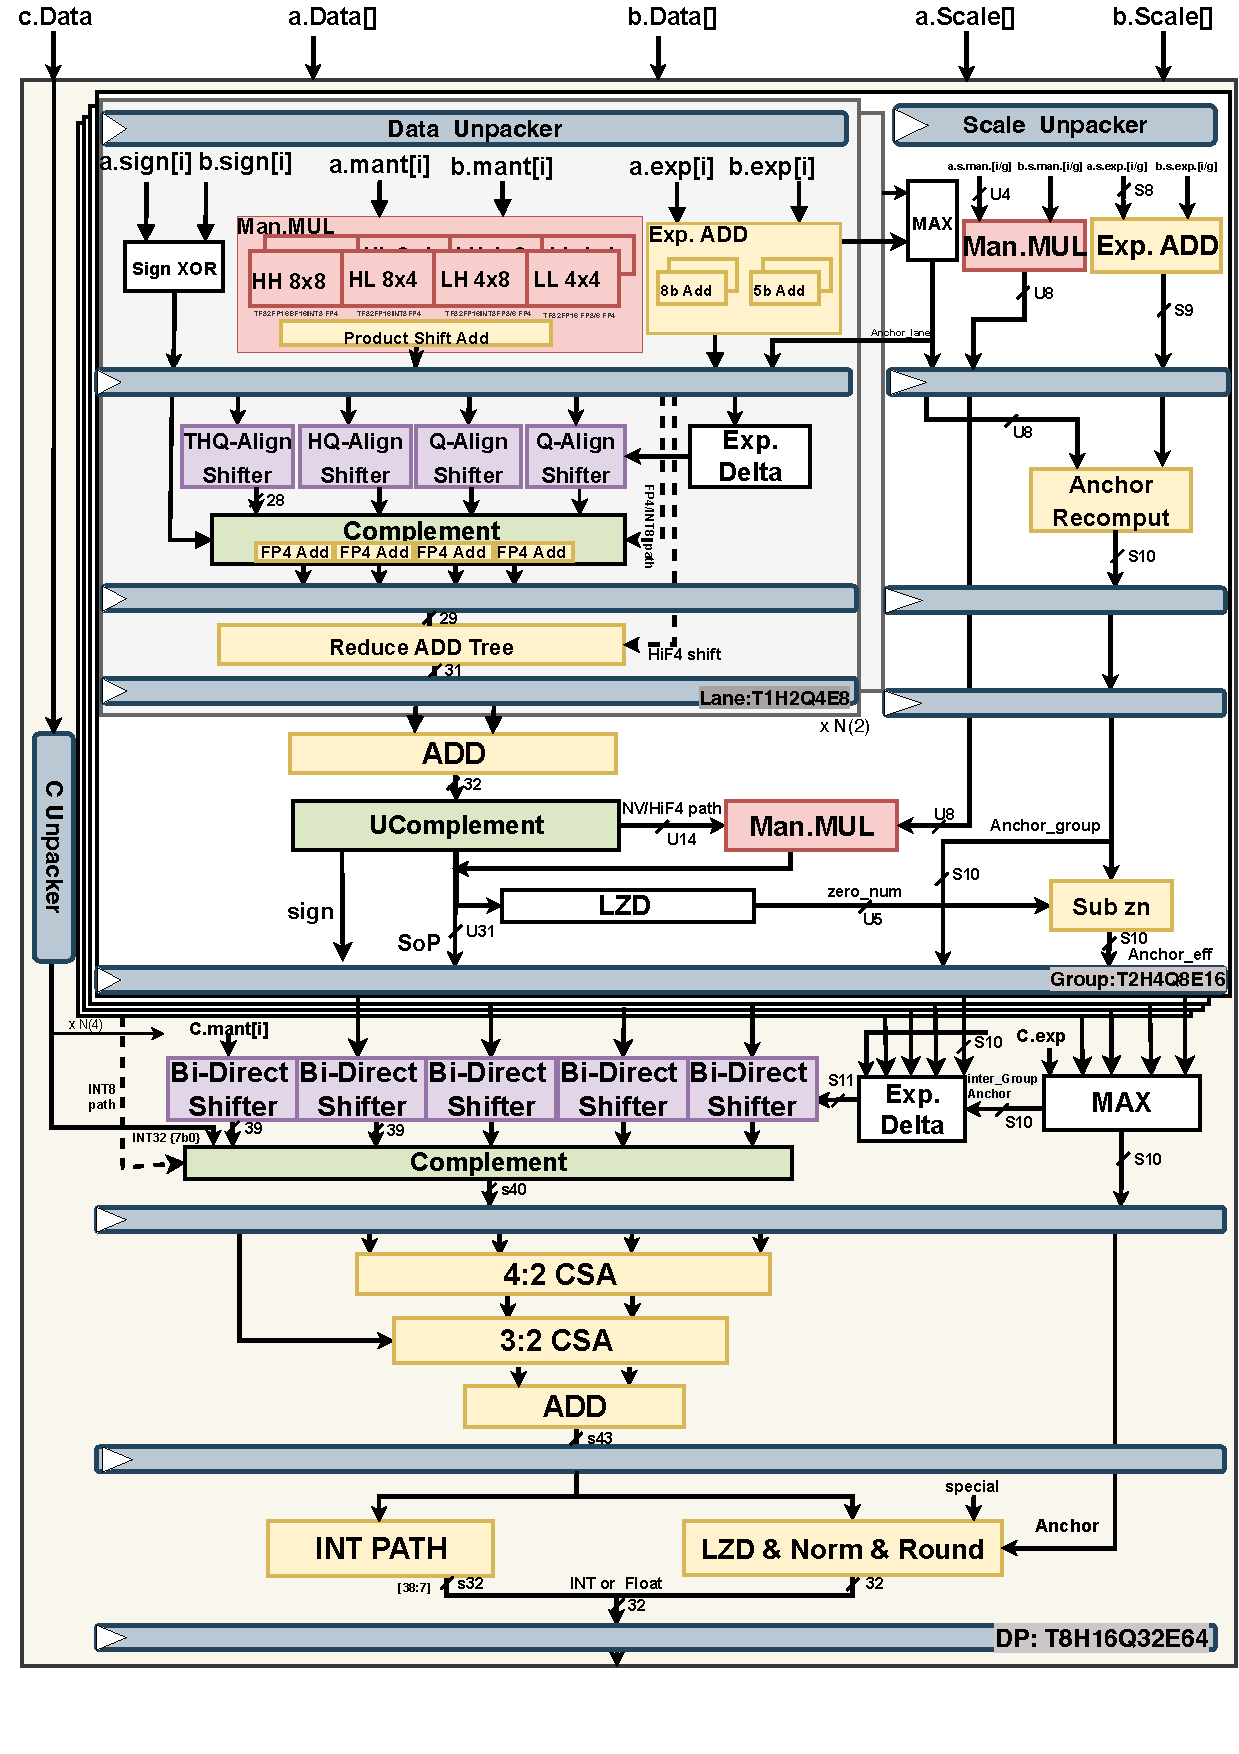
\includegraphics[width=0.90\linewidth,height=0.84\textheight,keepaspectratio]{baseline_arch.pdf}
\caption{\ratio{1}{2}{4} 基线点积单元。Lane 共享乘法及局部规约，Group 合并两条 Lane 并施加块尺度，DP 对齐各组部分和与 $C$ 后完成累加。}
\label{fig:baseline}
\end{figure}

如图~\ref{fig:baseline} 所示，计算通路划分为 Lane、Group 和 DP 三层。T 指 TF32，H 指 FP16/BF16，Q 指 MXFP8/6，E 指 MXFP4/NVFP4/HiF4。每条基线 Lane 在不同模式下的容量分别为 T1H2Q4E8，另支持 4 对 INT8 输入。两条 Lane 组成 T2H4Q8E16 Group，四个基线 Group 组成 T8H16Q32E64 DP，INT8 容量为 32。浮点算力配比以 H:Q:E 的 16:32:64 归一化为 \ratio{1}{2}{4}。这些是同一套硬件在互斥模式下的峰值，统一按 1 次乘加计 1 MAC。

从算术上看，若一个块的 A、B 解码值分别写成 $s^{(A)}_g u_i$ 与 $s^{(B)}_g v_i$，块内点积为
\begin{equation}
  q_g=s^{(A)}_g s^{(B)}_g\left(\sum_{i\in g}u_i v_i\right).
\end{equation}
尺度乘法由此从每对元素的一次计算变成对块部分和的一次调节。当一个尺度块覆盖多个物理组时，对应计算组使用相同的尺度，跨组继续规约。HiF4 的局部微指数计入每项 $u_i$、$v_i$ 或 Lane 的定点和，组级接口承担其中的外层尺度。这个组织同时满足格式的块划分与流水中的并行度。

\subsubsection{输入格式、块尺度与物理分组}

\begin{figure}[!htbp]
\centering
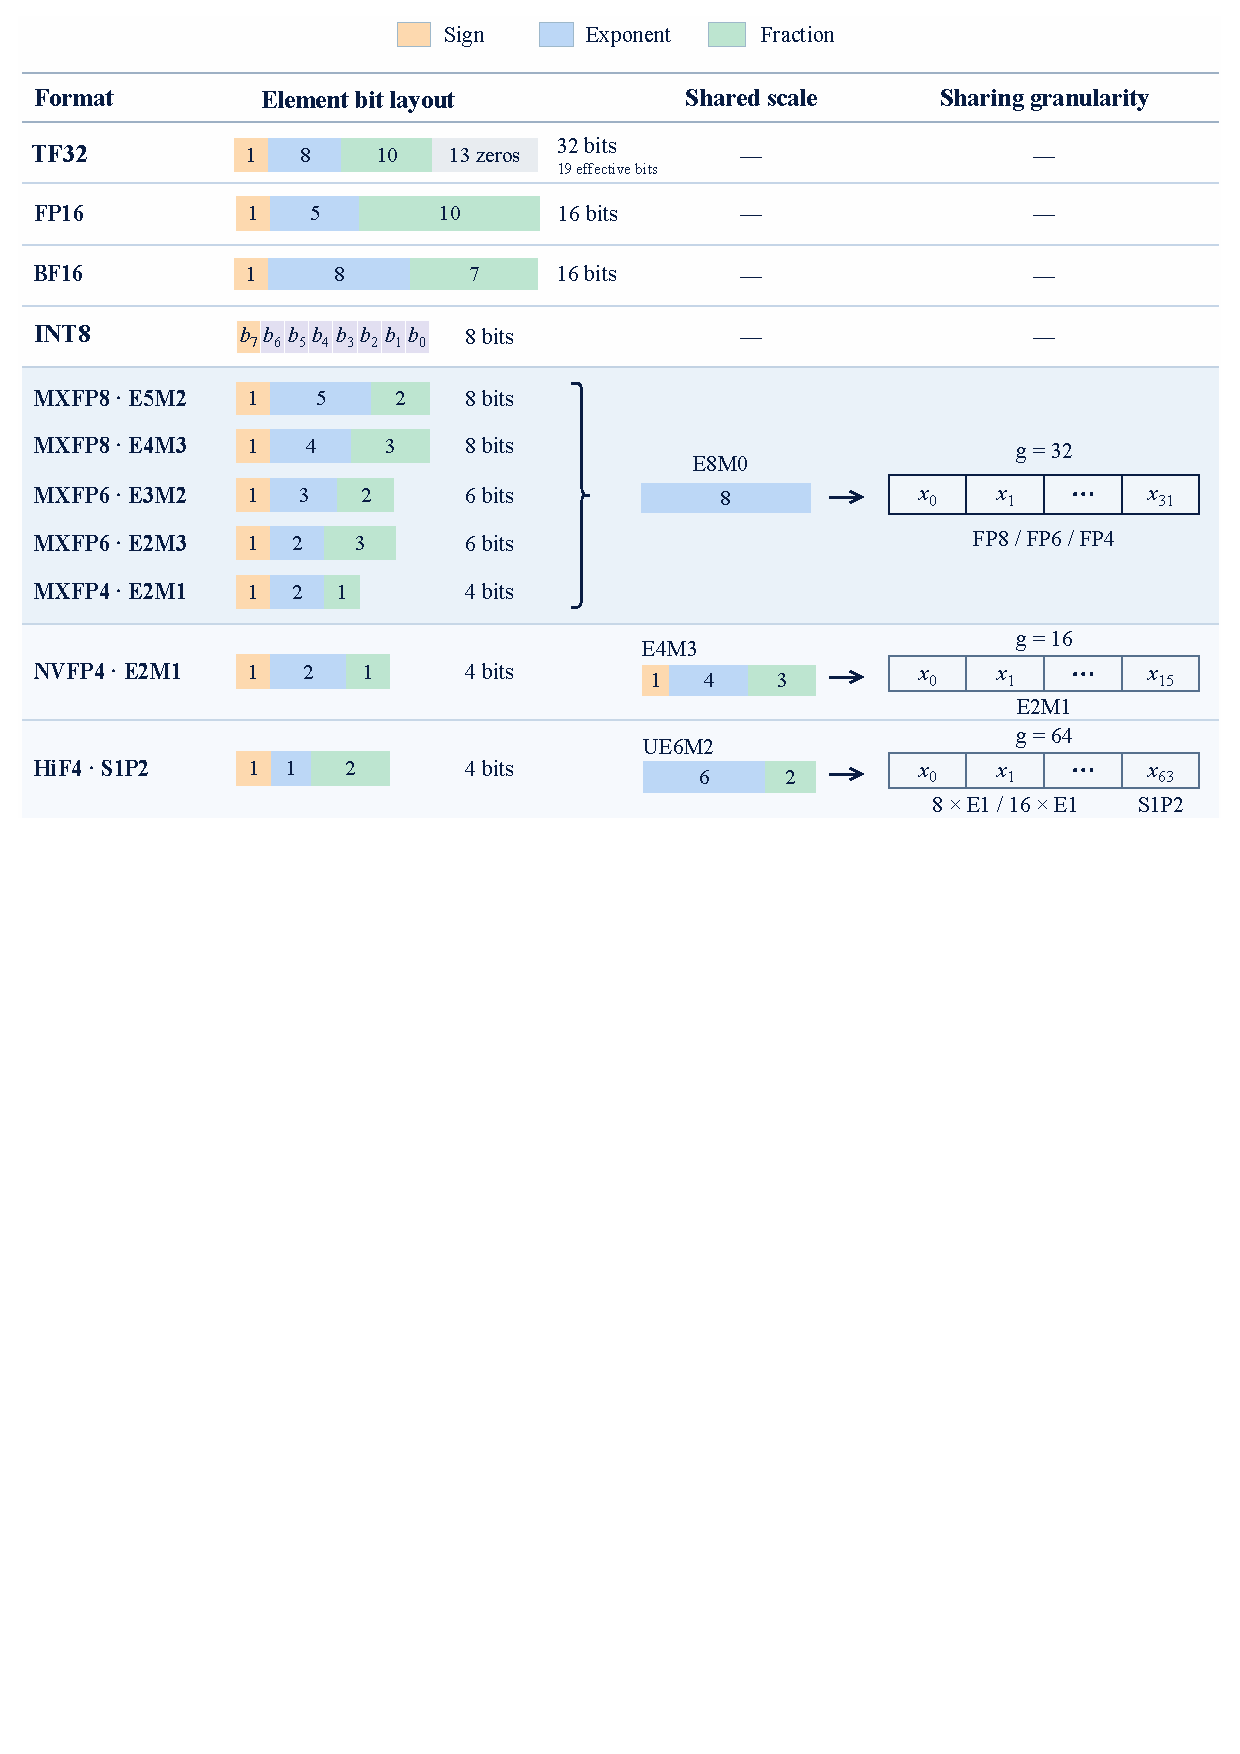
\includegraphics[pagebox=cropbox,width=0.88\linewidth]{image/formate.drawio.pdf}
\caption{点积单元支持的元素编码与块尺度。MX、NVFP4 与 HiF4 的尺度粒度决定了尺度与 Lane、Group 的对应关系。}
\label{fig:dp-formats}
\end{figure}

图~\ref{fig:dp-formats} 给出了元素与尺度的含义。TF32 在 32 位槽内携带 8 位指数和 10 位尾数字段，低 13 位为零。FP16 与 BF16 占用相同的 16 位槽，但前者为 5 位指数和 10 位尾数字段，后者为 8 位指数和 7 位尾数字段。四种 MXFP8/6 的指数位与尾数字段分配各异，以 32 元素共享的 E8M0 表示块尺度。MXFP4 和 NVFP4 共享 E2M1 元素编码，前者沿用 MX 的 32 元素二次幂尺度，后者为每 16 元素配置 E4M3 尺度。HiF4 在 64 元素上共享 UE6M2 基准尺度，每 4 元素一位一级微指数，每 8 元素一位二级微指数。INT8 则以二补码表示整数。这些差异分别影响乘法器位宽、局部对齐和尺度处理，不能仅凭码字位数划分通路。

每条 Lane 从 A、B 两侧各接收 32 位元素载荷，基线 DP 每侧总计 256 位。尺度和微指数走独立旁带，A、B 的格式一致，但两侧使用各自的元数据。划分为两 Lane 一组后，E16 Group 的边界同时对齐两个 HiF4 二级微指数块和一个 NVFP4 尺度块。大于 Group 的尺度块只需将同一尺度分发给相邻组。例如，$K=96$ 的 HiF4 沿六个 E16 Group 分配为 $(s_0,s_0,s_0,s_0,s_1,s_1)$，相同长度的 MXFP4 分配为 $(s_0,s_0,s_1,s_1,s_2,s_2)$。增加 Group 因而只改变输入分发和后端参加规约的组数，内部算术可以复用。$C$ 与 A、B 同拍输入，由本笔请求保留至全局累加。矩阵计算需要分多笔处理时，由上层把前一笔对应输出坐标的 $D$ 作为后一笔的 $C$。

\subsection{输入重编码与乘法器复用}

\subsubsection{Lane 内的定宽解包}

\begin{figure}[!htbp]
\centering
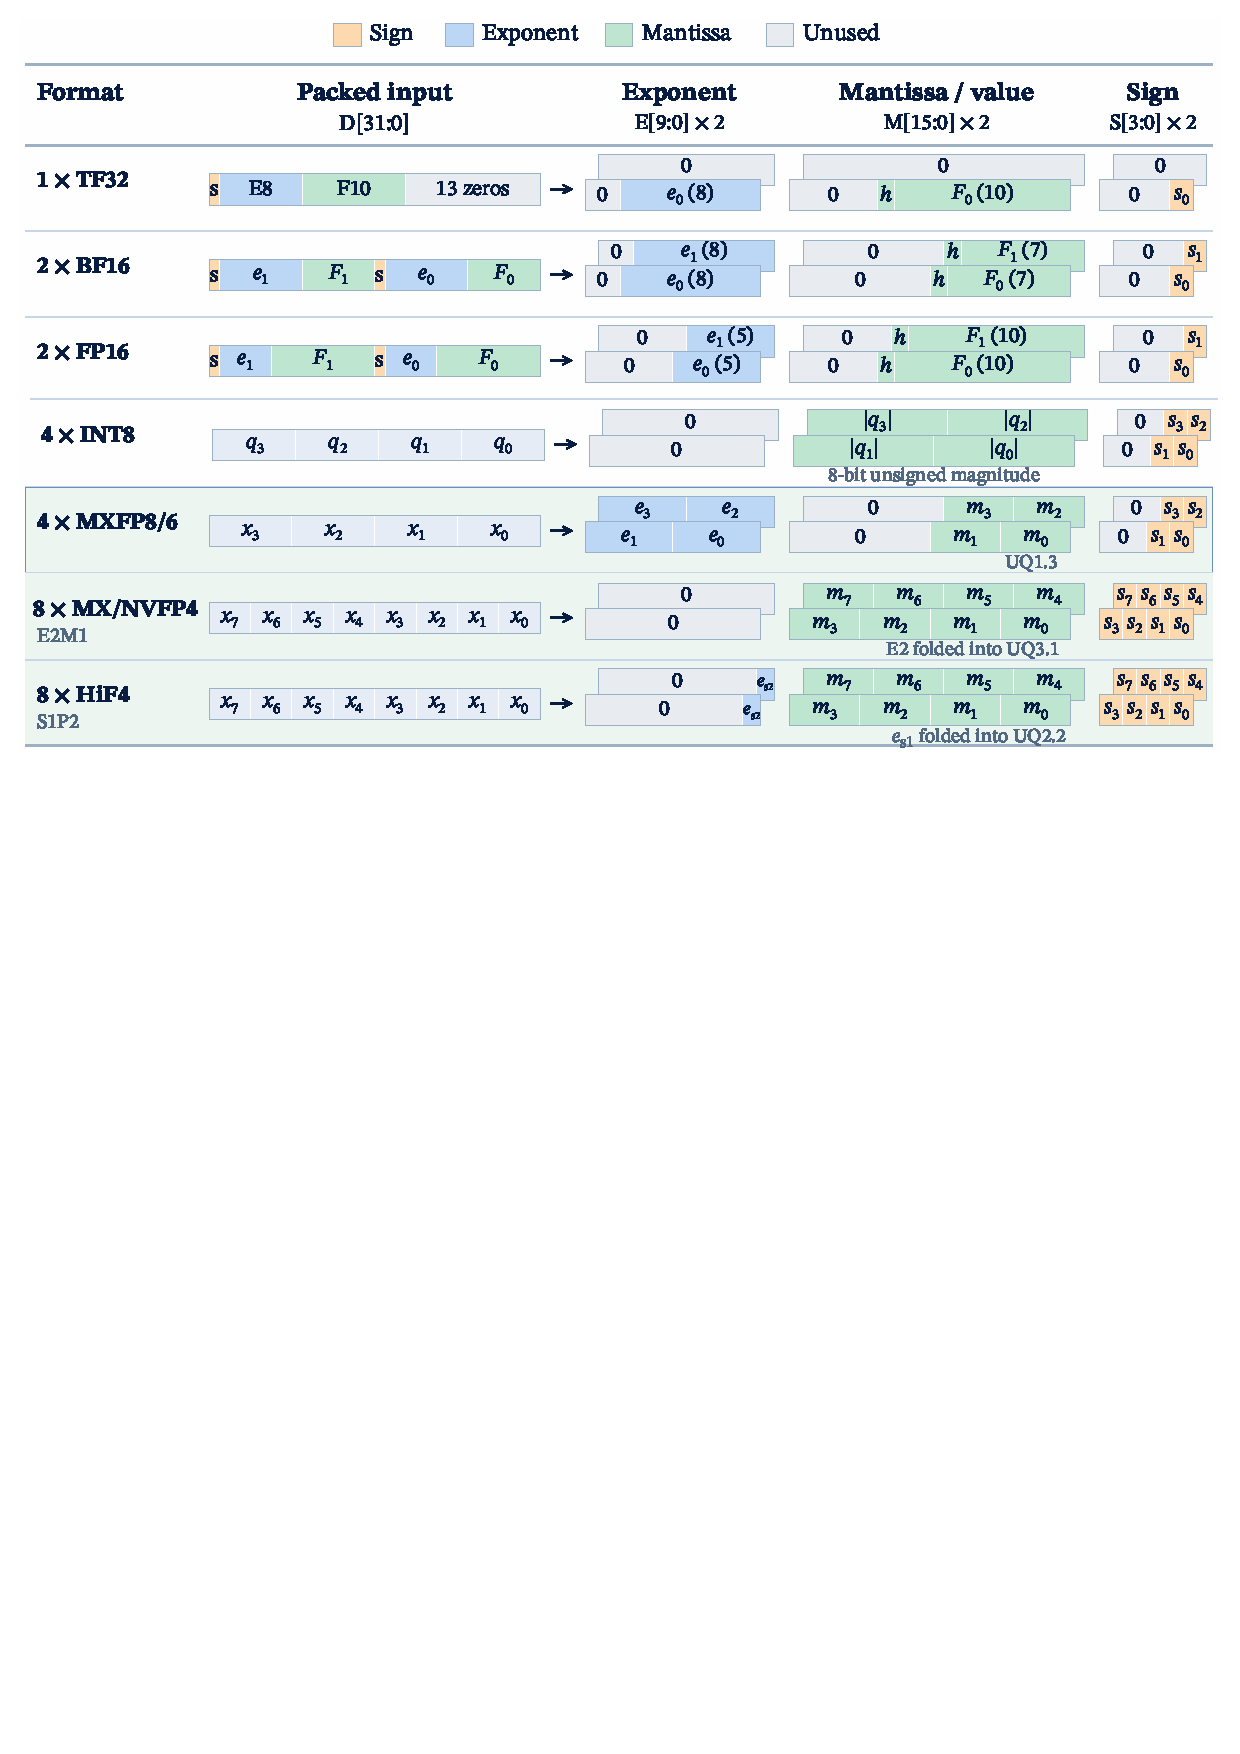
\includegraphics[pagebox=cropbox,width=0.94\linewidth]{image/unpack.pdf}
\caption{基线 Lane 的输入解包。每侧 32 位载荷按格式整理为两组内部符号、指数、幅值记录，TF32 只激活其中一组。}
\label{fig:dp-unpack}
\end{figure}

如图~\ref{fig:dp-unpack} 所示，S1 以 16 位为基本槽，将一侧 32 位输入重排成两条定宽记录。每条记录用 4 位符号、10 位指数和 16 位幅值容纳当前模式的子元素。TF32 跨两个槽但只产生一个有效元素，H 模式每槽一个，Q 模式每槽两个，E 模式每槽四个，INT8 每槽两个。FP6 的六位编码占用字节的高六位，剩余两位为零，内部算术仅使用原编码。这样的组织把槽位抽取、符号分离、指数修正和尾数填充集中在乘法之前，后续固定宽度的路由无需再解析原始格式。

T/H 路径用隐含位和尾数字段组成无符号定点系数。对于次正规值，隐含位清零，指数仍取最小正规指数，以保留有效幅值。Q 路径将 2 位或 3 位尾数字段精确嵌入统一的 UQ1.3 坐标。设原码的尾数字段和指数域分别为 $f$、$e$，尾数字段宽度为 $b$，格式的指数偏置为 $B$，则有限值的解包满足
\begin{equation}
  h=\mathbf{1}_{e\ne0},\qquad
  m=\bigl(h\,2^b+f\bigr)2^{3-b},\qquad
  e'=\max(e,1)+(15-B),\qquad
  x=(-1)^s m\,2^{-3}2^{e'-15}.
  \label{eq:q-unpack}
\end{equation}
例如，E5M2 和 E4M3 对 $1.25$ 的编码不同，经式~\eqref{eq:q-unpack} 均得到 $m=10$、$e'=15$。该转换只改定点坐标和偏置，元素已有的有效位全部保留。零、无穷和 NaN 按各格式规则分类，特殊标志与幅值并行传递。

E2M1 的八种非负幅值 $\{0,0.5,1,1.5,2,3,4,6\}$ 对应 UQ3.1 的整数系数 $\{0,1,2,3,4,6,8,12\}$。HiF4 将三位 S1P2 幅值系数按一级微指数 $e_1$ 左移，最大为 $7\times2=14$，可以用 UQ2.2 的四位系数表示。二级微指数在同一 Lane 内共享，留到局部求和后使用。因此，三种 E 格式都可通过四位幅值乘法实现精确的元素乘积，且无需为每项单独保存和比较乘积指数。

\subsubsection{由同一组部分积覆盖宽乘积与窄乘积}

基线每条 Lane 含两套乘法单元，每套各有一个 $8\times8$、$8\times4$、$4\times8$ 和 $4\times4$ 乘法器。TF32、FP16 的尾数含隐含位共 11 位。将尾数写为 $a=a_h2^4+a_l$、$b=b_h2^4+b_l$，并将高片段零扩展至 8 位，则一套硬件的四个部分积按原位权重构
\begin{equation}
  ab=(a_hb_h)2^8+(a_hb_l+a_lb_h)2^4+a_lb_l .
  \label{eq:mul-reconstruct}
\end{equation}
交叉项相加保留增长位，有效 11 位输入产生完整的 22 位乘积，含 20 位小数。BF16 的 8 位有效尾数可直接使用主乘法器计算，结果保留 14 位小数。Q 模式使用独立的四位幅值，乘积有 6 位小数。E 模式将独立的元素对送入每套的四个乘法器，宽端口高位补零，因此各结果只含当前元素对的乘积。INT8 将 $-128$ 转成符号和绝对值 128。每套可用主乘法器计算一个整数乘积，将另一对的 B 操作数拆成高、低四位，通过两条交叉乘法路径及一次固定左移拼成第二个完整的 $8\times8$ 乘积。

\begin{table}[!htbp]
\centering
\caption{基线 Lane 的模式路由和局部对齐需求}
\label{tab:lane-routing}
\zihao{5-}
\begin{tabularx}{\linewidth}{@{}lrYr@{}}
\toprule
模式 & 元素对数 & 两套乘法资源的使用方式 & 可变移位路数 \\
\midrule
TF32 & 1 & 一套启用四个部分积并重构，另一套隔离 & 1 \\
FP16 & 2 & 每套启用四个部分积，分别重构一个宽乘积 & 2 \\
BF16 & 2 & 每套使用 $8\times8$ 主乘法器 & 2 \\
MXFP8/6 & 4 & 每套计算两个独立的窄乘积 & 4 \\
MXFP4/NVFP4/HiF4 & 8 & 每套的四个乘法器分别计算四个窄乘积 & 0 \\
INT8 & 4 & 每套用主乘法器和交叉部分积生成两个整数乘积 & 0 \\
\bottomrule
\end{tabularx}
\end{table}

表~\ref{tab:lane-routing} 表明，乘法器复用的代价集中在输入选通、宽乘积重构及随流水传递的模式控制。以 BF16 为例，两个主乘法器足以完成运算，其余部分积单元的输入保持隔离，可以减少无效翻转。相比为每类格式分别铺设乘法器，这一组织用同一物理资源实现宽格式的完整位权和窄格式的多元素并行。

\subsection{移位器复用与组部分和的位宽}

\subsubsection{T/H/Q 组内指数对齐}

同一组的元素乘积在施加块尺度前，先在共同二进制坐标下规约。S2 在两条 Lane 的有效有限非零项中选择最大乘积参考指数 $r$。两条 Lane 因此共用一个对齐坐标，S5 合并 Lane 和时可直接相加。设乘积为 $P_i$，默认保留 26 位小数，则坐标的最小量化单位 $\Delta_{\mathrm{loc}}$ 及对齐系数 $q_i$ 可写为
\begin{equation}
  \Delta_{\mathrm{loc}}=2^{r-26},\qquad
  q_i=\operatorname{sgn}(P_i)\left\lfloor
                  \frac{|P_i|}{\Delta_{\mathrm{loc}}}\right\rfloor .
  \label{eq:local-align}
\end{equation}
TF32、FP16 的 20 位乘积小数先以低位补零纳入 28 位幅值窗口，BF16 和 Q 也保持各自的原乘积位权。指数差产生的右移发生在该公共坐标下，幅值截断后再恢复符号，对正负值均相当于向零截断。发生丢位时，单项截断的绝对误差小于 $\Delta_{\mathrm{loc}}$。符号恢复后每个叶子占 29 位，四项 Lane 和保留为 31 位，两 Lane 合并再增长一位。

不同模式只改变四个通用移位器的启用数，T/H/Q 分别使用 1、2、4 路。高精度格式需要处理跨度更大的指数差，Q 格式需要更多并行通道，两类需求由相同的四路移位网络覆盖。每个乘积在局部对齐时预留的小数位越多，相消时保留下来的低位越多，同时移位器、加法树和数据寄存器也会随之增宽。本文采用的 28 位局部幅值与 40 位全局有符号叶子，是后续验证和综合实验的默认配置。

\subsubsection{E 路径的定点规约与块缩放}

E 模式不使用乘积指数最大值及四路可变移位器。每条 Lane 的八个乘积恢复符号后，先两两相加形成四个 10 位有符号数，再进入共享四叶加法树，得到 12 位有符号和。MXFP4、NVFP4 的乘积有两位小数，树和通过低位补两个零映射到四位小数坐标。HiF4 乘积已有四位小数，将树和扩位后按 $p=e_{2,A}+e_{2,B}\in\{0,1,2\}$ 左移即可。把微指数移位移到树后，因为 Lane 内八项所乘的 $2^p$ 相同，只需一次小位移。HiF4 的最大系数和为 $8\times14^2\times 2^2=6272$，MXFP4 和 NVFP4 为 $8\times12^2\times2^2=4608$，均可放入 14 位有符号坐标。两 Lane 合并时保留 15 位，取绝对值后的组和幅值为 14 位。INT8 的四个乘积也按固定整数坐标进入规约。

块缩放分开处理尺度的指数和系数。MX 的 E8M0 尺度直接加到组的指数，幅值旁路。NVFP4 与 HiF4 的两侧尺度各以四位定点系数承载，先在 S2 计算 $4\times4$ 系数积，得到小数位数为 6 的八位结果。S5 在 E 窄通路计算 $14\times8$ 组幅值乘法，得到含 10 位小数的 22 位幅值。尺度指数在解包时统一为无偏值，S2 求和，并在 S3 与组坐标常量合成最高物理位的指数候选。等到 S5 实际幅值就绪，便可直接计算供后端使用的比较指数。E 专用组在 22 位上完成前导零检测，输出低补九个零嵌入公共 31 位幅值。补零同时移动了小数点，指数坐标随之保持等价，因此不会改变数值。由此可在保留 FP4 块缩放的前提下，让扩展组以窄幅值进入公共后端。

\subsection{融合累加与全局舍入}

$C$ 参与全局对齐的时机决定了哪些低位信息能留到最终结果。以数学点积等于 $1+2^{-24}$、$C=-1$ 为例，若点积先被舍入为 FP32，最近偶数舍入会将中点结果记为 $1$，再与 $C$ 相加得到零。若内部位宽能够一直保留该低位，先与 $C$ 求和会留下可精确表示的 $2^{-24}$。因此本文让 $C$ 与缩放后的组部分和共同进入末端规约。这样的融合结构只在最后形成 FP32 编码，有限窗口内的移位截断仍按前述数值合同发生。

组接口包括符号 $s$、31 位幅值 $u$、最高物理位的指数 $a_{\mathrm{raw}}$，以及供比较的指数 $a_{\mathrm{cmp}}$。幅值实际表示 $(-1)^s u\,2^{a_{\mathrm{raw}}-30}$。若 $u$ 具有 $z$ 个前导零，非零 Group 的最高有效位指数为 $a_{\mathrm{cmp}}=a_{\mathrm{raw}}-z$。例如，某组的物理最高位指数为 $5$ 而其前导零数为 $3$，该组只会将全局参考指数提高至 $2$。这使全局窗口能容纳更多有意义的低位。S6 先从比较指数中选出公共指数 $E_\star$，再依据 $E_\star-a_{\mathrm{raw}}$ 对原幅值作一次双向移位。差值为正时右移，为负时左移。这样既可按真实有效位比较，也省去组幅值先规格化再对齐的两次移位。

$C$ 在 S5 解包。正规数采用编码指数，非正规数用 $-126$ 作为比较上界并保留原幅值，省去 $C$ 侧的前导零检测。这个上界可能高于 $C$ 实际最高有效位的指数，测试用例因此包含最小、最大非正规 $C$ 与结果相消的情形。$C$ 已经处于输出数值坐标，直接参与全局对齐，无需施加 A、B 的块尺度。默认全局对齐叶子为 40 位有符号数。

基线四个 Group 先经 4:2 压缩为和、进位两行，再与唯一的 $C$ 通过 3:2 压缩。$C$ 可以与组部分和走同一位权选择及末端加法器，组内乘积对齐也无需为一个动态范围更大的 FP32 输入预留多套通路。扩展组同样在对齐后形成两行，和基线两行合并。按当前精度选择基础两行或合并两行，再经唯一的进位传播加法器（Carry-Propagate Adder，CPA）得到完整总和。设当前顶层最多有 $G$ 个 Group，求和位宽取 $40+\lceil\log_2(G+1)\rceil$，其中 $1$ 对应 $C$。五输入基线保留 43 位，最多有 17 个输入的配置保留 45 位。进位保存结构推迟了进位传播，避免扩展部分求和与最终求和形成串联的宽 CPA。尾级对总和取幅值并检测前导零，用共同指数及首个有效位位置恢复 FP32 指数。RNE 根据保留位之后的首个舍入位、其余低位的并集以及保留尾数的最低位判定是否进位。舍入进位使尾数溢出时再调整指数。

精度切换要求算术使能与请求一同推进。每个组分别记录该请求是否使用该组，以及参与项是否有限非零。后者用于指数最大值和数值移位，前者用于特殊值及负零的规则。例如，E 请求在扩展组留下 NaN 后，紧随其后的 H 请求停用该组，残留 NaN 应从特殊值规约中移除。反过来，当前 E 请求的 NaN 虽然没有有限幅值，仍须传到输出。这个区分也使停用组不会在负零规约中被误认为参与的正零。

\begin{table}[htbp]
\centering
\caption{基线八级流水及主要数值边界}
\label{tab:pipeline}
\zihao{5-}
\begin{tabularx}{\linewidth}{@{}lYY@{}}
\toprule
流水级 & 主要运算 & 数值边界 \\
\midrule
S1 & 元素和尺度解包，传递原始 $C$ & 符号与幅值分离，尺度指数转为无偏值 \\
S2 & 幅值乘法，组内有效指数比较，尺度系数预乘 & E 绕过元素指数最大值，保留定点乘积 \\
S3 & T/H/Q 幅值对齐，E 乘积两两规约 & 局部 RTZ，预计算组幅值坐标 \\
S4 & Lane 四项树规约，基线和 QE 融入 HiF4 二级微指数 & E 定点和统一为四位小数坐标 \\
S5 & 两 Lane 合并、块缩放与前导零检测，解包 $C$ & 形成公共组幅值、物理位指数与比较指数 \\
S6 & 所有活动组和 $C$ 的公共指数对齐 & 单次双向移位及符号恢复 \\
S7 & 进位保存压缩、精度选择及 CPA & 按输入数保留求和增长位，$C$ 计入一次 \\
S8 & 规格化、RNE、特殊值或整数回绕 & FP32 或 INT32 输出 \\
\bottomrule
\end{tabularx}
\end{table}

表~\ref{tab:pipeline} 给出基线流水。E 专用组将窄树提早收敛，在 S3 完成二级微指数融合，S4 做组和及取幅值，S5 做块缩放和 22 位前导零检测。不同配置的接口延迟均为 8 拍，启动间隔 $\mathrm{II}=1$。例如，周期 $n$ 接收的一笔请求在 $n+8$ 产生结果，周期 $n+1$ 可接收另一种格式。有效位随流水传递，数据寄存器在本级有效且当前模式启用时更新。各配置保持相同的发射和接收规则，便于阵列统一调度。

\subsection{专用 Group 与算力配比构造}

扩展组与基线使用相同的部分和接口，其差异主要位于 S1--S5。E16 专用组保留每条 Lane 八个 $4\times4$ 乘法器，裁去 T/H/Q/INT8 解码、元素指数比较和宽对齐。窄规约使 Lane 和由共享通路的 31 位减为 14 位。Q8 专用组每条 Lane 保留四个 $4\times4$ 乘法器和 Q 的指数对齐，裁去 E 的解码、微指数及尺度尾数乘法。Q8E16 每条 Lane 保留八个 $4\times4$ 乘法器，Q 模式用四个，E 模式用八个。它同时保留 Q 的宽对齐与 NVFP4/HiF4 的尺度处理，E 模式旁路宽移位并复用规约树。因此，是否需要 Q 的逐元素指数对齐决定了 E16 与 Q8E16 的规约位宽，而 Q8 只适合增加 FP8/6 吞吐。

设附加的 Q8、E16、Q8E16 数量分别为 $g_Q$、$g_E$、$g_{QE}$。各模式的原生归约长度为
\begin{equation}
  K_H=16,\qquad K_Q=32+8(g_Q+g_{QE}),\qquad
  K_E=64+16(g_E+g_{QE}).
  \label{eq:ratio-groups}
\end{equation}
由于各配置每拍发射一笔，式~\eqref{eq:ratio-groups} 也给出单个输出位置各模式的峰值 MAC/cycle。Q8E16 的两个峰值来自同一物理资源在不同模式下的使用。构造配比时，保持 H 吞吐为基准，通过增减不同类型的 Group 来单独或联合扩大 Q、E 算力。

% 组数来自 dp-puzzle_dac2027/tables/group_compositions.tex 与 src/spec/dp/dptop/。
\begin{table}[htbp]
\centering
\caption{九种算力配比的 Group 组成}
\label{tab:groups}
\zihao{5-}
\begin{tabular}{@{}lrrrrl@{}}
\toprule
H:Q:E & 基线 Group & Q8 & E16 & Q8E16 & 浮点原生并行度 \\
\midrule
\ratio{1}{2}{4}  & 4 & 0 & 0  & 0  & T8H16Q32E64 \\
\ratio{1}{2}{6}  & 4 & 0 & 2  & 0  & T8H16Q32E96 \\
\ratio{1}{2}{8}  & 4 & 0 & 4  & 0  & T8H16Q32E128 \\
\ratio{1}{4}{4}  & 4 & 4 & 0  & 0  & T8H16Q64E64 \\
\ratio{1}{4}{8}  & 4 & 0 & 0  & 4  & T8H16Q64E128 \\
\ratio{1}{2}{12} & 4 & 0 & 8  & 0  & T8H16Q32E192 \\
\ratio{1}{2}{16} & 4 & 0 & 12 & 0  & T8H16Q32E256 \\
\ratio{1}{6}{12} & 4 & 0 & 0  & 8  & T8H16Q96E192 \\
\ratio{1}{8}{16} & 4 & 0 & 0  & 12 & T8H16Q128E256 \\
\bottomrule
\end{tabular}
\end{table}

表~\ref{tab:groups} 中，两个 E16 将 $K_E$ 由 64 增至 96，对应 \ratio{1}{2}{6}，四个 E16 则使其翻倍，对应 \ratio{1}{2}{8}。若希望以相同数目的附加组同时将 $K_Q$ 从 32 增至 64，可改用四个 Q8E16，得到 \ratio{1}{4}{8}。这三个实现覆盖仅增加 E 与联合增加 Q/E 的两种思路。较大的候选继续增加相应组数，用于观察归约更宽时节约的计算时间能否覆盖面积和功耗代价。新增组有各自的对齐入口，复用末端规格化和舍入。

本阶段还实现了独立 E64 和 Q32E64，分别由四个 E16 和四个 Q8E16 构成。把这些单元接成额外的输出列，可以在保留基线原生 $K$ 的同时获得较高的 FP4 或 Q/E 算力。两种办法由此共用已验证的 Group，但分别增加每个输出内的乘积数和每拍输出数。第~\ref{sec:dse} 节在相同配比下比较两者的单元成本与接口载荷，再对同构 $K$ 扩展阵列进行九种配比的预算扫描。

\subsection{Golden 模型、测试向量和验收指标}

\subsubsection{独立数学参考与有限位宽期望}

验证对同一笔端口编码计算精确数学结果和有限位宽结果。数学参考由独立的 Python 程序生成。该程序按格式独立解码 A、B、$C$、块尺度及 HiF4 微指数，把每个有限值表示为有理数。逐项计算 A 与 B 对应元素的乘积并累加 $C$，仅在末端按 IEEE 754 的 FP32 RNE 规则编码\cite{ieee754,Goldberg1991}。例如，精确结果若恰位于 FP32 相邻编码的中点，参考程序比较精确余数，按较低候选的最低有效位决定是否进位。NaN、无穷、零及其符号按格式规则分类。INT8 则在整数域累计，再取低 32 位，与硬件回绕语义对照。

导入数据时保留原有 FP64 参考，并重算精确期望。这样可以识别由中间累加引入的 FP64 双重舍入。例如，在一笔 $K=64$ 的 MXFP8 E4M3 扩展向量中，精确和位于一个 FP32 舍入分界点的一侧，FP64 路径给出的 FP32 编码与精确参考相差 1 ULP。24 套扩展语料共 23064 笔，重算后发现 14 笔有限输出存在这类 1 ULP 差异。先解析数学真值再比较有限位宽实现，可以把原有 FP64 路径的舍入差异与硬件丢位区分开来。

有限位宽期望按流水中的实际舍入与丢位规则计算。C++ CModel 逐级实现指数比较、两级定点对齐、向零截断、尺度乘法、压缩求和与最终舍入，先用独立的 Python 有限窗口参考校验，再以 CModel 导出的期望逐位检查冻结 Verilog，逐级比对内部断点。这样一来，RTL 即使与数学参考只相差 1 ULP，只要偏离已验证的有限窗口期望，仍会被判为实现错误。反过来，RTL 与有限窗口期望一致后，再统计其相对数学参考的误差，用以评价位宽选择。

\subsubsection{测试向量的来源和覆盖}

九种基础浮点编码各有 961 笔数据，依次包括 64 笔随机、128 笔混合随机、256 笔和 512 笔来自模型输入分布的向量及一笔全一输入。扩展数据的两个模型分布段分别取自 DeepSeek 和 Qwen 负载。随机样本覆盖比模型样本更广的编码和指数差；模型样本用来观察激活与权重按真实分布组合时的误差；全一输入便于直接检查不同配比的原生 $K$、组使能及累加次数。TF32 和 INT8 采用固定种子 20271104，各生成 512 笔编码随机和 512 笔有限值或累加器边界输入，另加定向极值和全一输入，分别共 1053 和 1045 笔。

扩展配置按原生 $K$ 保留完整的 A、B、$C$、分块尺度和微指数，覆盖 Q 的 $K=64,96,128$ 及 E 的 $K=96,128,192,256$。导入器按元素逻辑索引及格式块边界映射端口。例如，HiF4 在 $K=96$ 时，前 64 与后 32 个元素各使用本段尺度。这样可以检查最后两个物理组是否正确继承第二个尺度，而不会因把 $K=64$ 输入简单复制而掩盖错误。每套数据记录样本顺序、源数据校验和、尺度槽映射及参考程序版本，同一份向量由 CModel 与 RTL 共同读取。

数值以外的协议检查按输入序号记录预期结果和到达时刻，并比对输出数值、类型和流末标记。测试覆盖连续发射、逐拍换型、气泡和复位取消。基线另有 5314 笔新增定向向量，覆盖 FP4 编码乘积、HiF4 局部尺度及相消、块尺度边界和非正规 $C$，共检查 1095599 个 S1--S7 内部断点。混合配置还有停用组保留大指数、特殊值和负零的用例，以及 27/40、28/40、32/64 三组局部和全局窗口的协议与断点检查。某一级若出现差异，可沿解包、局部规约、块尺度、全局对齐顺序找到首次失配，即使个别中间错误碰巧在末端相消也能检出。

\subsubsection{ULP 度量与分格式结果}

ULP（Unit in the Last Place）是浮点数末位的间隔。对于 FP32，在正规区间 $[2^e,2^{e+1})$ 上，相邻正数差 $2^{e-23}$。为了给跨指数和跨符号的结果定义统一距离，设 $m$ 为去掉符号位的 FP32 编码，$b=2^{31}$，有限值的序号取为 $b+m$（非负）或 $b-m$（负号），两个有限结果的 ULP 距离为序号差的绝对值。$+0$ 与 $-0$ 在距离度量中同点，协议仍可单独检查零的符号。NaN、Inf 及 INT32 分别按分类或编码合同处理。

对齐截断误差还可按绝对值估算。式~\eqref{eq:local-align} 给出单项局部丢位上界，乘以该组的尺度积后即可换回最终数值坐标。全局截断按公共对齐坐标的量化单位界定，最后计入 RNE 的半间距舍入误差。绝对误差与 ULP 同时报告具有实际意义，因为严重相消时，较小的绝对误差在零附近仍可能跨过较多编码。混合顶层对原生语料设定 4 ULP 回归检查线，工程验收仍以 RTL 与有限位宽期望逐位相同为准。

% 分格式结果来自 test/results/mixed-rtl-v1.9.json 的 baseline 记录。
\begin{table}[!htbp]
\centering
\caption{基线 DP 的分格式精确数学参考结果}
\label{tab:numeric-by-format}
\zihao{5-}
\begin{tabular}{@{}lrrr@{}}
\toprule
格式 & 向量数 & 与数学参考逐位一致 & 最大 ULP \\
\midrule
TF32 & 1053 & 1040 & 1 \\
FP16 & 961 & 949 & 1 \\
BF16 & 961 & 958 & 3 \\
MXFP8 E5M2 & 961 & 958 & 1 \\
MXFP8 E4M3 & 961 & 961 & 0 \\
MXFP6 E3M2、E2M3（各） & 961 & 961 & 0 \\
MXFP4、NVFP4、HiF4（各） & 961 & 961 & 0 \\
INT8 & 1045 & 1045 & -- \\
\midrule
合计 & 10747 & 10716 & 3 \\
\bottomrule
\end{tabular}
\end{table}

% 数据来自 test/results/mixed-rtl-v1.9.json 与 five-expansions-final-v1.12-20261112.json。
\begin{table}[htbp]
\centering
\caption{Verilator 冻结 RTL 原生数据验证结果}
\label{tab:numeric}
\zihao{5-}
\begin{tabular}{@{}lrrr@{}}
\toprule
H:Q:E & 与有限位宽期望逐位一致/总数 & 与数学参考逐位一致 & 最大 ULP \\
\midrule
\ratio{1}{2}{4} & 10747/10747 & 10716 & 3 \\
\ratio{1}{2}{6} & 10747/10747 & 10715 & 3 \\
\ratio{1}{2}{8} & 10747/10747 & 10716 & 3 \\
\ratio{1}{4}{4} & 10747/10747 & 10710 & 3 \\
\ratio{1}{4}{8} & 10747/10747 & 10710 & 3 \\
\ratio{1}{2}{12} & 10747/10747 & 10714 & 3 \\
\ratio{1}{2}{16} & 10747/10747 & 10716 & 3 \\
\ratio{1}{6}{12} & 10747/10747 & 10714 & 3 \\
\ratio{1}{8}{16} & 10747/10747 & 10714 & 3 \\
\ratio{0}{2}{4} & 6727/6727 & 6724 & 1 \\
\ratio{0}{0}{4} & 2883/2883 & 2883 & 0 \\
\bottomrule
\end{tabular}
\tabnote{最大 ULP 按浮点结果统计，逐位一致数含 INT8。九个全精度配置均覆盖 11 种编码，均通过 L8、II=1 及定向协议检查。}
\end{table}

表~\ref{tab:numeric} 汇总各配置的原生输入验证。基线的 31 笔数学参考差异集中于 TF32、FP16、BF16 和 MXFP8 E5M2，详见表~\ref{tab:numeric-by-format}。三种 E 格式在基线上各有 961 笔与数学参考完全一致，部分扩展配置的 MXFP4 或 NVFP4 出现 1 ULP 偏差。归约长度增加后，更多组部分和落在同一个全局窗口，仍可能发生全局丢位。这里的最大距离是本批向量在给定位宽下的观测值。

\subsection{综合与真实负载功耗评估}
\label{sec:ppa}

\subsubsection{评估流程与工况}

对通过 Verilator 功能与协议验收的 Verilog 单元冻结源文件并记录内容指纹。使用 Synopsys Design Compiler X-2025.06 在 TSMC 12\,nm、TT、0.7\,V、85\,\textcelsius 下进行逻辑综合和工艺映射。目标时钟为 1\,GHz，时钟转换时间为 0.10\,ns，开启集成时钟门控（ICG）。在同一工艺和约束下比较各配置的组合逻辑、寄存器及门控单元面积，并检查时序、电气与映射库约束。代表性配置的建立与保持检查见表~\ref{tab:timing}。基线和扩展的最差建立裕量接近零，因此本节时序与面积采用综合后工况，留待布局布线阶段复核长路径和扇出。

\begin{table}[htbp]
\centering
\caption{代表性配置的 1\,GHz 综合时序裕量}
\label{tab:timing}
\zihao{5-}
\begin{tabular}{@{}lrr@{}}
\toprule
H:Q:E & 建立裕量（ps） & 保持裕量（ps） \\
\midrule
\ratio{1}{2}{4} & 0.001311 & 1.306176 \\
\ratio{1}{2}{6} & 0.000477 & 0.395805 \\
\ratio{1}{2}{8} & 0.011325 & 0.175148 \\
\ratio{1}{4}{4} & 0.000119 & 0.024334 \\
\ratio{1}{4}{8} & 0.006318 & 0.083819 \\
\bottomrule
\end{tabular}
\end{table}

\subsubsection{负载构造与门级活动采样}

功耗输入来自 Qwen3-8B 在 WikiText-2 上推理时第 0 层 MLP 下投影。从该层采集实际中间激活和下投影权重，沿归约维选择相应片段构成 A、B。同一模式下按各 DP 的原生 $K$ 取样，保留量化后的端口编码、块尺度及微指数；同源样本保留共同的参考前缀累加值作为 $C$。这里的 $C$ 以 FP32 表示，由 BF16 参考计算提供。各笔输入是独立的点积切片，可以持续发射。按真实张量取样可以保留零值、指数及相邻输入翻转的统计特征，也使不同 $K$ 的测量建立在有对应关系的输入上。

设计综合后以同一份约束、映射网表与工艺单元仿真模型进行门级重放。基线三种模式各有 1024 笔负载，先进行合法初始化，再发射全部负载，冻结 RTL 与网表的输出均与有限位宽期望逐位对照。发射的前 256 笔用于预热，第 256 至 767 笔的发射时间段以 VCS X-2025.06-1 提取原生 SAIF。在 1\,GHz 且每拍发射一笔时该区间为 512\,ns。末段继续发射并排尽流水，以核对全部负载的结果。窗口位于连续发射中部，有助于避开复位、起流水和排空时的短时活动变化。

SAIF 记录各节点的逻辑状态驻留时间和翻转次数。例如，节点在测量区间 $T_w$ 内翻转 $N_{\mathrm{tog}}$ 次，平均翻转率为 $N_{\mathrm{tog}}/T_w$。Power Compiler X-2025.06 将活动映射回综合网表，对端口、网络和单元引脚做注释覆盖审计。基线实测三点的显式注释率均为 100\%，实际引脚的未知及高阻状态驻留为零。审计同时核对真实引脚的翻转率和概率，使停用通路的零翻转能够被保留，而不会被缺省活动覆盖。

% 基线功耗来源 hw/power/records/baseline_v18_repaired_1109.csv。
% 功能功耗来源 figure/H16Q32E64_power/power.csv。
\begin{table}[!htbp]
\centering
\caption{基线 DP 的分模式功耗与每 MAC 能量}
\label{tab:baseline-power}
\zihao{5-}
\setlength{\tabcolsep}{4.5pt}
\begin{tabular}{@{}lrrrrrrr@{}}
\toprule
 & & \multicolumn{5}{c}{功耗（mW）} & \\
\cmidrule(lr){3-7}
模式 & $K$ & 内部 & 切换 & 动态 & 漏电 & 总计 & pJ/MAC \\
\midrule
BF16         & 16 & 11.551 & 3.636 & 15.187 & 0.141 & 15.328 & 0.958 \\
MXFP8 E4M3   & 32 & 12.100 & 3.760 & 15.860 & 0.142 & 16.002 & 0.500 \\
MXFP4 E2M1   & 64 &  8.586 & 2.469 & 11.055 & 0.141 & 11.197 & 0.175 \\
\bottomrule
\end{tabular}
\tabnote{动态功耗为内部功耗和负载切换功耗之和，总功耗计入漏电。表中各列独立舍入。}
\end{table}

表~\ref{tab:baseline-power} 给出三种代表模式的分项。MXFP4 的每拍乘积数是 BF16 的四倍，但其总功耗约为 BF16 的 73\%，与其旁路局部可变移位、使用窄规约以及停用宽乘积重构的设计一致。按同一网表的功能分项，对齐与移位在 BF16、MXFP8 和 MXFP4 下分别约为 3.14、3.32、1.49\,mW。比较不同 $K$ 时，以每拍实际完成的 MAC 为分母，即 $E_{\rm MAC}=P_{\rm total}\,\mathrm{II}/(Kf)$。MXFP8 的对齐路数是 BF16 的两倍，总功耗略高。由于每拍计算更多乘积，其每 MAC 能量约为 BF16 的一半。功耗对应综合后零延迟单 DP 的活动，时钟树、布线寄生与延迟引发的毛刺将在后端实现中评估。

\subsubsection{基线 DP 的功能面积划分}

表~\ref{tab:baseline-area} 将完成综合和电气规则检查的基线映射网表按功能展开。使用映射后叶单元面积，经功能层次和网表节点与来源逻辑的对应关系分类。每个叶单元只归入一个类别，同一功能所属的寄存、选择和控制逻辑随其主体计入。多功能复用或归属不唯一的少量逻辑计入其他。七类小计与综合报告的 $16165.122154\,\mu\mathrm{m}^2$ 总面积一致到表中显示精度，既可用于核对，也可用于判断扩展某一模式时哪些电路能裁减。

% 基线面积来自 figure/H16Q32E64_area/area.csv 的 dp_top 行。
\begin{table}[!htbp]
\centering
\caption{\ratio{1}{2}{4} 基线 DP 的综合面积按功能划分}
\label{tab:baseline-area}
\zihao{5-}
\begin{tabularx}{\linewidth}{@{}lYrr@{}}
\toprule
功能 & 主要电路 & 面积（$\mu\mathrm{m}^{2}$） & 占比（\%） \\
\midrule
乘法 & 元素部分积与重构、尺度系数乘法、组幅值乘尺度 & 3903.345 & 24.15 \\
求和与累加 & Lane 和 Group 的规约树、组间压缩、最终 CPA & 3530.760 & 21.84 \\
对齐与移位 & 组内和全局移位、指数差及局部定点移位 & 2758.939 & 17.07 \\
数据解包 & A/B、块尺度及 $C$ 解包与相应寄存 & 2590.286 & 16.02 \\
指数处理 & 指数运算、最大值比较与范围处理 & 1808.253 & 11.19 \\
规格化与舍入 & 前导零检测、规格化、舍入和结果封装 & 490.844 & 3.04 \\
其他 & 公共控制、门控、旁带及其余共享逻辑 & 1082.696 & 6.70 \\
\midrule
合计 & & 16165.122 & 100.00 \\
\bottomrule
\end{tabularx}
\tabnote{面积和百分比按未舍入的叶单元小计计算，展示值独立舍入。}
\end{table}

乘法、求和与累加、对齐移位合计占约 63.1\%。其中，单独的对齐与指数处理占约 28.3\%，解释了 E 扩展为何将消除逐乘积指数比较和可变移位与缩窄规约树结合起来，仅缩小乘法器只能降低部分增量开销。数据解包约占 16.0\%，反映出多格式支持需要承担槽位重排、指数重编码和元数据分发。规格化与舍入仅占约 3.0\%，因为多条局部通路在形成部分和后共同使用一个输出转换级。这三处结构取舍分别作用于格式接入、局部资源和输出后端，构成表~\ref{tab:ppa} 中不同扩展方案的成本差异。

\subsubsection{面积、功耗与扩展代价}

% 数值来源 figure/DP_area_power/dp11_area_power_fixed_20261116.csv。
% 九个 DSE 项的原始记录索引见 ratio_dse/dse/inputs/provenance.json。
\begin{table}[htbp]
\centering
\caption{各配比单个 DP 的综合面积和负载总功耗}
\label{tab:ppa}
\zihao{5-}
\begin{tabular}{@{}lrrrrr@{}}
\toprule
 & & & \multicolumn{3}{c}{总功耗（mW）} \\
\cmidrule(l){4-6}
H:Q:E & 面积（$\mu\mathrm{m}^2$） & 面积增幅（\%） & BF16 & MXFP8 & MXFP4 \\
\midrule
\ratio{1}{2}{4} & 16165.12 & 0.00 & 15.328 & 16.002 & 11.197 \\
\ratio{1}{2}{6} & 18863.27 & +16.69 & 15.637 & 16.354 & 14.417 \\
\ratio{1}{2}{8} & 21596.41 & +33.60 & 15.893 & 16.620 & 17.595 \\
\ratio{1}{4}{4} & 24015.38 & +48.56 & 15.943 & 26.909 & 11.683 \\
\ratio{1}{4}{8} & 27191.14 & +68.21 & 15.744 & 28.789 & 20.563 \\
\ratio{1}{2}{12} & 26620.01 & +64.68 & 15.821 & 16.550 & 23.463 \\
\ratio{1}{2}{16} & 29692.81 & +83.68 & 16.063 & 16.636 & 29.382 \\
\ratio{1}{6}{12} & 38234.35 & +136.52 & 15.977 & 41.351 & 29.747 \\
\ratio{1}{8}{16} & 46925.55 & +190.29 & 16.287 & 52.853 & 38.906 \\
\ratio{0}{2}{4} & 11695.21 & -27.65 & -- & 13.580 & 10.218 \\
\ratio{0}{0}{4} & 5644.14 & -65.08 & -- & -- & 7.036 \\
\bottomrule
\end{tabular}
\tabnote{面积增幅以 \ratio{1}{2}{4} 为基准。\ratio{0}{2}{4} 与 \ratio{0}{0}{4} 为专用对照，横线处无对应模式。两种最大 Q/E 联合扩展的 PPA 引用投稿归档数据。}
\end{table}

\begin{figure}[htbp]
\centering
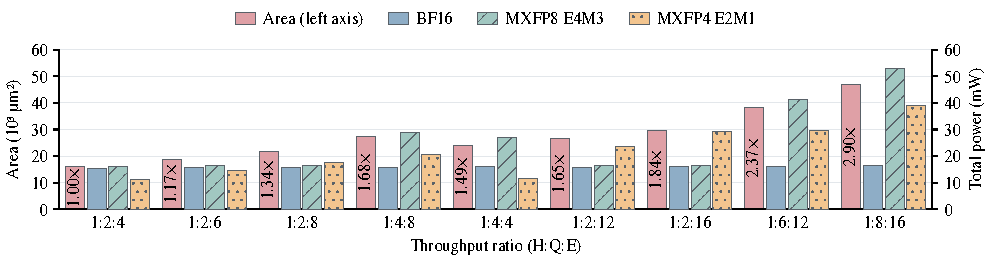
\includegraphics[width=\linewidth]{dp_ratio_area_power.pdf}
\caption{九种全精度配比的单 DP 面积与分模式功耗。面积和功耗分别按左、右轴读取。}
\label{fig:ppa}
\end{figure}

\textbf{FP4 单独扩展所需面积低于同等倍数的 FP8 扩展。}
以 \ratio{1}{2}{4} 为基准，FP4 翻倍的 \ratio{1}{2}{8} 增加 33.60\% 面积，FP8 翻倍的 \ratio{1}{4}{4} 增加 48.56\%。E16 将固定点重编码和窄规约的优势保留在物理实现中，Q8 则仍需元素指数比较、移位和宽加法树。在相同的 FP4 原生 $K=64$ 下，独立 E64 和 Q32E64 的 MXFP4 总功耗分别为 7.04 和 10.22\,mW，基线为 11.20\,mW。这组对照反映了复用所需的宽寄存器、选择和公共后端仍有开销。基线的功能面积构成见表~\ref{tab:baseline-area}。

\textbf{Q/E 共享可以减少两种吞吐同时扩大的增量面积。}
把 FP8、FP4 独立扩展的面积增量相加，得到基线面积的 82.16\%。采用四个 Q8E16 同时使两类吞吐翻倍时，\ratio{1}{4}{8} 的增幅为 68.21\%，相当于在上述两项增量之和的基础上节约 16.98\%。此比较以独立扩展的增量之和为参照，体现了乘法复用与公共数据通路摊销带来的面积收益。

\textbf{单位计算能量和峰值功耗给出不同的预算信号。}
\ratio{1}{2}{8} 的 MXFP4 总功耗由 11.197 增至 17.595\,mW，其吞吐由 64 增至 128\,GMAC/s，单位面积吞吐提高约 49.70\%，每 MAC 能量由 0.17495 降至 0.13746\,pJ，降幅 21.43\%。在基线 BF16、MXFP8、MXFP4 三种条件下，最大功耗为 16.002\,mW，由 MXFP8 决定。\ratio{1}{2}{8} 的最大功耗改由 MXFP4 决定，较基线最大值增加 9.95\%。当 Q 和 E 同时扩展时，\ratio{1}{4}{8} 的最大功耗升至 28.789\,mW，由 MXFP8 决定，相对基线最大值增加 79.91\%。九种设计的 BF16 功耗增长均在 6.3\% 以内。不同模式的活动功耗直接决定预算内可同时开启的 DP 数量。

\section{阵列组织及预算约束下的配比分析}
\label{sec:dse}

\subsection{同构与异构阵列实现同一配比}
\label{sec:array-choices}

点积单元增加低精度吞吐后，阵列可以在两个维度利用新增资源。以 $D_{M\times N}=A_{M\times K}B_{K\times N}+C_{M\times N}$ 为例，$K$ 表示同一输出位置的归约长度，$N$ 表示输出列数。阵列每周期的有效乘加数取决于活动输出位置数与每个位置的原生 $K$。因此，在相同的 $M$ 并行度下，将原生 $K$ 或活动 $N$ 增为两倍，都可以实现该模式峰值算力翻倍。两种方案复用的对象不同，外部接口也相应变化。

\textbf{同构 DP 阵列沿 $K$ 扩展。}
阵列中的每个输出位置均采用同一配置的扩展 DP。以 \ratio{1}{2}{8} 为例，每个位置从 T8H16Q32E64 换成 T8H16Q32E128，低精度扩展组计算同一输出的额外 64 对 FP4 元素。新增组的部分和在 DP 内归并，整个位置共享一个 $C$ 接口和输出规格化器。FP4 模式下每笔请求应送入更长的 A 行片段和 B 列片段，输出坐标数仍为 $M_0N_0$。若若干归约片段可在一次原生操作中合并，还能减少一部分跨请求的累加读写。高精度模式下各位置保持相同的原生长度，调度仍覆盖同一个输出网格。

\textbf{异构 DP 阵列沿 $N$ 扩展。}
保留基线 DP 的输出列，在同一阵列增加由 E64 或 Q32E64 组成的专用列。对于 \ratio{1}{2}{8}，一列基线 DP 与一列 E64 在 FP4 模式下分别计算两个不同的输出位置，各取 64 对操作数。相同的 A 行片段可以广播给新增列，B 侧则按输出列提供不同的权重片段。每个新位置要保存自己的累加状态并产生独立结果，因而扩大的是输出侧的 C/D 通路。此处 $C$ 是输入累加值，$D$ 是写回的更新值，在 Cube 内二者通常对应同一累加存储的读、写两侧。\ratio{1}{4}{8} 可以用相同办法给基线列配对 Q32E64，使 Q、E 模式均增加输出位置，高精度计算仍由基线列承担。

设基线每拍覆盖 $M_0$ 行、$N_0$ 列和 $K_0$ 项归约，比较将某个低精度模式的峰值翻倍的两种方案。表~\ref{tab:array-traffic} 按阵列供数边界上的独立逻辑元素计数，假定行广播与列广播充分复用，C/D 每次需要读写的值按输出位置计。以 FP4 的 \ratio{1}{2}{8} 为例，取 $K_0=64$，同构 DP 每个位置消费 $128$ 对元素，异构两个位置各消费 $64$ 对，表中结论可直接应用到两者。

\begin{table}[htbp]
\centering
\caption{等峰值低精度扩展下的阵列数据量对照}
\label{tab:array-traffic}
\begin{tabular*}{0.94\linewidth}{@{\extracolsep{\fill}}lcccc@{}}
\toprule
阵列组织 & 每拍有效 MAC & A 输入元素 & B 输入元素 & C/D 各侧元素 \\
\midrule
基线 & $M_0N_0K_0$ & $M_0K_0$ & $K_0N_0$ & $M_0N_0$ \\
同构 DP，$K$ 翻倍 & $2M_0N_0K_0$ & $2M_0K_0$ & $2K_0N_0$ & $M_0N_0$ \\
异构 DP，活动 $N$ 翻倍 & $2M_0N_0K_0$ & $M_0K_0$ & $2K_0N_0$ & $2M_0N_0$ \\
\bottomrule
\end{tabular*}
\tabnote{表中为满利用、等发射间隔时每笔 tile 事务的载荷。换算为带宽需乘对应元素位宽及发射率，并计入块尺度。累加驻留在片内时，C/D 流量主要落在片内累加存储及端口。}
\end{table}

在这组配对条件下，B 的元素需求都翻倍，因此区分两种方案的首先是 A 侧广播复用和 C/D 侧读写。若限制来自 A 缓冲读口，复用同一行片段的 $N$ 扩展更容易供数，但广播的扇出变大。若 C/D 端口或局部累加容量已经接近上限，$K$ 扩展可以把额外乘积留在同一输出位置内合并。以 FP4 的 \ratio{1}{2}{8} 为例，阵列供数侧的一行 A 在 $K$ 扩展下每拍多读 64 个低精度元素及其尺度，而在 $N$ 扩展下，该行片段新增一个广播接收列。对应地，$N$ 扩展每增加一个活动输出位置，就多一次 32 位 $C$ 的供给和一次 32 位 $D$ 的接收。若这些值驻留在片内，额外需求体现为累加器容量和更新端口。实际 GEMM 还有尾块效应。$N$ 较窄时专用列可能缺少有效输出，$K$ 较短或频繁遇到块边界时加宽的归约通路也可能用不满。表~\ref{tab:array-traffic} 由此给出需要在阵列中测量的方向，跨 tile 访存、双缓冲与累加驻留将在调度模型中计入。

\subsection{等吞吐点的计算单元成本}

表~\ref{tab:kn-local} 采用实测单 DP 数据比较两种阵列组织的算术单元小计。以一个基线输出位置为参照，同构方案取一个扩展 DP，异构方案取一个基线 DP 加一个专用 DP。只比较两种方案均能满载的扩展模式。这样，\ratio{1}{2}{8} 的 FP4 均为每拍 128 MAC，\ratio{1}{4}{8} 的 FP8、FP4 分别均为每拍 64、128 MAC。面积按单元相加，功耗按相应模式活动总功耗相加。

\begin{table}[htbp]
\centering
\caption{等低精度吞吐下的计算单元面积与活动功耗}
\label{tab:kn-local}
\begin{tabular*}{0.9\linewidth}{@{\extracolsep{\fill}}llrrr@{}}
\toprule
配比 & 实现与数据口径 & 面积（$\mu\mathrm{m}^2$） & FP8（mW） & FP4（mW） \\
\midrule
\ratio{1}{2}{8} & $K$ 扩展 DP（综合与功耗评估） & 21596.41 & -- & 17.595 \\
                 & $N$ 扩展，基线 + E64（单元相加） & 21809.26 & -- & 18.233 \\
\ratio{1}{4}{8} & $K$ 扩展 DP（综合与功耗评估） & 27191.14 & 28.789 & 20.563 \\
                 & $N$ 扩展，基线 + Q32E64（单元相加） & 27860.34 & 29.582 & 21.414 \\
\bottomrule
\end{tabular*}
\tabnote{原始单元数据见表~\ref{tab:ppa}。$N$ 列数据为计算单元组合估计，尚需计入阵列广播、累加端口、存储体、布线及门控。横线所示模式在这组方案中维持基线吞吐。}
\end{table}

两个等吞吐点中，按独立单元相加得到的 $N$ 扩展面积较 $K$ 扩展高约 0.99\% 和 2.46\%，已比较的活动功耗高约 2.76\%--4.14\%。$K$ 扩展共用一套输出对齐、累加和舍入电路，新增部分和需要进入更宽的组间规约网络。$N$ 扩展各列保留独立后端，但额外列可选用更窄的专用 DP。这两项成本相互抵消，使所得计算单元小计接近。配比实现的选择因而需要进一步比较阵列数据流。下文先在同构 $K$ 扩展条件下分析九种配比，把可独立选择专用列的 $N$ 扩展留作下一阶段的同条件系统比较。

\subsection{同构阵列下从单 DP 数据推导可用算力}

在同构阵列中，同一配比的每个输出位置安装同一种 DP。由于阵列形状与每核输出位置数保持相同，可用九种 $K$ 扩展 DP 的综合面积和分模式总功耗计算各候选的部署规模与可用算力。设 $j$ 为候选配比，$p\in\{H,Q,E\}$ 为当前计算模式，$A_j$ 为单 DP 面积，$P_{j,p}$ 为其活动功耗，$I_j$ 为空闲功耗代理，取三种活动报告中的最大漏电。每个候选核心采用 $D_{\mathrm{core}}=256$ 个相同 DP。以 \ratio{1}{2}{4} 为基线，设 $N_0=36$ 核，基准 DP 阵列面积占核心面积的比例 $\alpha=0.327$。该比例参考公开的昇腾计算簇面积研究\cite{luo2024hifloat8area}，用于标定本节分析场景。设每核的外围存储和控制面积固定，则等面积预算下的物理核数为
\begin{equation}
  N_j=\left\lfloor\frac{N_0}{1+\alpha(A_j/A_0-1)}\right\rfloor.
  \label{eq:physical}
\end{equation}
阵列功耗预算按基线全核在三种已测精度中的最大活动功耗设定
\begin{equation}
  B=\beta N_0 D_{\mathrm{core}}\max_p P_{0,p}.
  \label{eq:powerbudget}
\end{equation}
当 $\beta=1$ 时，功耗上限约为 147.47\,W。每种精度下允许开启的核数 $n_{j,p}$ 分别计算，取满足以下约束的最大整数
\begin{equation}
  D_{\mathrm{core}}\bigl[n_{j,p}P_{j,p}+(N_j-n_{j,p})I_j\bigr]\le B,
  \qquad 0\le n_{j,p}\le N_j .
\end{equation}
模型用空闲代理保留未开启核的漏电项，并采用固定频率 1\,GHz。每个模式的可用计算速率为
\begin{equation}
  R_{j,p}=\frac{2f D_{\mathrm{core}} K_{j,p} n_{j,p}}{\mathrm{II}} .
  \label{eq:rate}
\end{equation}
这里浮点乘法与加法分别计 1 FLOP，故每 MAC 计 2 FLOP。式~\eqref{eq:physical} 刻画面积对物理核数的影响，式~\eqref{eq:rate} 还纳入模式功耗对活跃核数的限制。由此可以比较单 DP 吞吐增加后芯片可用算力实际增加了多少。

\subsection{DeepSeek-V4.1-Flash 工作量和迁移场景}

实验采用 DeepSeek-V4.1-Flash 的公开模型定义\cite{deepseekv41source}，按层展开一条 batch=1 冷启动预填充请求中的投影、混合专家（MoE）、主注意力与输出头等计算。稠密矩阵乘按 $2MNK$ 计数，并乘实际调用次数，注意力相关矩阵乘按该层可见的位置对数统计。以 32768-token 请求的首层 $q_{\mathrm{down}}$ 投影为例，$M=32768$、$N=1280$、$K=5120$，一次计算约 $4.295\times10^{11}$ FLOP。按算子记录形状、精度和工作量，再聚合为 H、Q、E 三类。FP32 单独统计，计算时间对比只覆盖映射到这三类 DP 的 GEMM。

\begin{table}[htbp]
\centering
\caption{五个累积精度迁移场景与请求加权计算量构成}
\label{tab:migration}
\zihao{5-}
\begin{tabularx}{\linewidth}{@{}lYrrr@{}}
\toprule
 & & \multicolumn{3}{c}{建模 GEMM 工作量占比（\%）} \\
\cmidrule(l){3-5}
场景 & 本场景新增的精度映射 & H & Q & E \\
\midrule
A & 原生精度映射，W4A8 路由专家计入 FP8 & 14.68 & 72.65 & 12.68 \\
B & 路由专家的 gate、up、down 迁至 FP4 & 14.68 & 29.47 & 55.85 \\
C & 主注意力 QK/PV 与分组输出投影迁至 FP8 & 0.03 & 44.12 & 55.85 \\
D & 共享专家、Q-up 与最终输出投影（O-up）迁至 FP4 & 0.03 & 19.86 & 80.10 \\
E & 主注意力 QK/PV 与分组输出投影进一步迁至 FP4 & 0.03 & 5.22 & 94.75 \\
\bottomrule
\end{tabularx}
\tabnote{B--E 各自在上一场景上修改所列算子，其余保持原映射。H/Q/E 的代表吞吐和功耗取 BF16、MXFP8 E4M3 和 MXFP4 E2M1。}
\end{table}

表~\ref{tab:migration} 的场景 A 从原模型的精度出发，W4A8 路由专家按 FP8 计算能力计费。场景 B 将路由专家归入 FP4。此后依次考察主注意力、输出投影及共享专家等算子向较低精度的迁移。公开的 DeepSeek 路由专家 W4A4 部署给出场景 B 的先例\cite{nvidiav41routed2026}。FlashAttention-3 和 SageAttention3 分别提供低精度注意力的实现依据\cite{flashattention3,sageattention3}。本阶段将这些精度分配作为场景输入，DeepSeek 模型上的逐算子精度可行性留在后续验证。

请求权重来自 FreeInference 的 2047 条会话首次请求\cite{nixon2026requests}。按输入长度划分上界为 1K 至 1M token 的 11 档，每档按上界展开模型工作量，按请求频数确定该档权重。例如，$(16\mathrm{K},32\mathrm{K}]$ 占 33.56\%。设 $L_b$ 和 $w_b$ 分别为长度档上界及请求权重，$W_{s,p}(L_b)$ 为场景 $s$、长度 $L_b$ 下精度 $p$ 的 FLOP 数。以阵列充分供数且满利用为条件，得到
\begin{equation}
  T_{j,s}=\sum_b w_b\sum_{p\in\{H,Q,E\}}\frac{W_{s,p}(L_b)}{R_{j,p}},
  \qquad
  \overline{T}_j=\frac{1}{5}\sum_{s=\mathrm{A}}^{\mathrm{E}}T_{j,s},
  \qquad
  S_j=\frac{\overline{T}_0}{\overline{T}_j}.
  \label{eq:dsetime}
\end{equation}
每档先估计计算时间，再按请求频率平均。五个迁移阶段等权表示本节的比较目标。长度上界近似保留了不同长度的工作量差异，同时使表中的绝对时间受分档影响。$S_j$ 衡量式~\eqref{eq:dsetime} 所覆盖的理想 GEMM 计算时间。

\subsection{配比选择的阶段性结论}

\begin{figure}[!htbp]
\centering
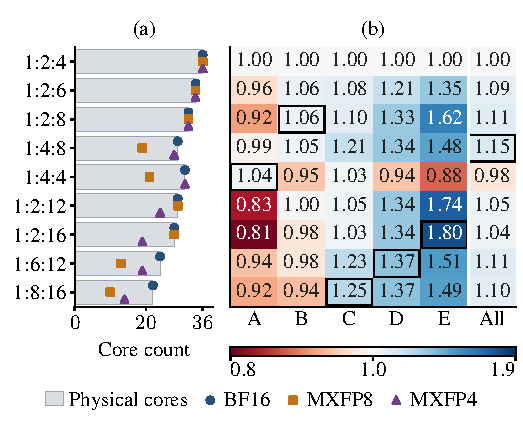
\includegraphics[width=0.62\linewidth]{five_scenarios_compare.pdf}
\caption{基准预算下，各配比的核数和分场景理想 GEMM 加速比。左图灰条为物理核数，三种标记为各模式活跃核数。右图 A--E 是五个迁移场景，All 为按式~\eqref{eq:dsetime} 汇总的结果。}
\label{fig:dse}
\end{figure}

% 数值来自本次用 ratio_dse/dse/study.json 重放的 fixed_scores.csv。
\begin{table}[htbp]
\centering
\caption{基准预算下的核数与五场景综合结果（$\alpha=0.327$，$\beta=1$）}
\label{tab:dse}
\zihao{5-}
\begin{tabular}{@{}lrrrrrr@{}}
\toprule
 & & \multicolumn{3}{c}{分模式活跃核数} & & \\
\cmidrule(lr){3-5}
H:Q:E & 物理核数 & H & Q & E & 计算时间（s） & 相对加速比 \\
\midrule
\ratio{1}{2}{4} & 36 & 36 & 36 & 36 & 3.3476 & 1.000 \\
\ratio{1}{2}{6} & 34 & 34 & 34 & 34 & 3.0792 & 1.087 \\
\ratio{1}{2}{8} & 32 & 32 & 32 & 32 & 3.0244 & 1.107 \\
\ratio{1}{4}{4} & 31 & 31 & 21 & 31 & 3.4283 & 0.976 \\
\ratio{1}{4}{8} & 29 & 29 & 19 & 28 & 2.9225 & 1.145 \\
\ratio{1}{2}{12} & 29 & 29 & 29 & 24 & 3.1781 & 1.053 \\
\ratio{1}{2}{16} & 28 & 28 & 28 & 19 & 3.2334 & 1.035 \\
\ratio{1}{6}{12} & 24 & 24 & 13 & 19 & 3.0053 & 1.114 \\
\ratio{1}{8}{16} & 22 & 22 & 10 & 14 & 3.0561 & 1.095 \\
\bottomrule
\end{tabular}
\end{table}



\textbf{在基准预算及五场景等权的设置下，\ratio{1}{4}{8} 的综合计算时间最短。}
表~\ref{tab:dse} 和图~\ref{fig:dse} 显示，\ratio{1}{4}{8} 的时间由基线的 3.3476\,s 降至 2.9225\,s，理想加速比为 $1.145\times$。该设计可部署 29 核，H、Q、E 各开启 29、19、28 核。相较只增加 E 算力的 \ratio{1}{2}{8}，该设计的每核 H、E 吞吐相同，可开启的 H、E 核数分别从 32 降至 29、28，因此两种模式的计算时间有所增加。Q 模式虽然从 32 个活跃核减少至 19 个，但原生 $K$ 从 32 增至 64，使全芯片 Q 吞吐由 524.3 提高到 622.6\,TFLOP/s。按式~\eqref{eq:dsetime} 对同一批工作量计算，缩短的 FP8 时间超过了 H 和 E 增加的时间。这解释了联合扩展在当前迁移权重下的优势，也指出了判断配比能否随工作量迁移而获益的方法。

\textbf{场景精度分布发生变化时，最优配比随之变化。}
在 A 中，Q 工作量占主导，\ratio{1}{4}{4} 居首，相对基线加速 $1.045\times$。只将路由专家迁至 FP4 的 B 中，\ratio{1}{2}{8} 居首，约为 $1.059\times$。在 E 中，主注意力和分组输出投影也迁至 FP4，\ratio{1}{2}{16} 居首，理想加速为 $1.801\times$。该设计在 FP4 下能开 19 核，单 DP 的原生 $K$ 为 256，按式~\eqref{eq:rate} 计算，全芯片 FP4 算力约为 2490.4\,TFLOP/s，\ratio{1}{4}{8} 对应约为 1835.0\,TFLOP/s。当 E 占比已经很高时，进一步增加 E 吞吐的收益可以覆盖其余模式吞吐下降的代价。

\textbf{可用阵列功耗越高，宽通路越有机会发挥峰值算力。}
对 $\alpha\in[0.25,0.50]$、$\beta\in[1,2]$ 做预算扫描。固定 $\alpha=0.327$，按 $\beta$ 以 0.1 分档，统计每档内获得最短时间的区间长度。\ratio{1}{4}{8} 在 $[1.0,1.1)$ 和 $[1.1,1.2)$ 两档的获胜区间占比最高，\ratio{1}{6}{12} 在 $[1.2,1.3)$ 和 $[1.3,1.4)$ 两档占比最高，\ratio{1}{8}{16} 在 $[1.4,2.0]$ 的各档领先。参考点的 \ratio{1}{8}{16} 可部署 22 核，FP8 和 FP4 仅能分别开启 10 核和 14 核，功耗上限放宽后才有更多物理核可用于低精度计算。

中文投稿稿件还保留了一套较严格的部署场景。该场景要求所有已部署核在任一已测模式下都能同时活动，并对 55 个迁移场景与长度组合等权，\ratio{1}{2}{8} 以约 $1.13\times$ 的加速居首。以 \ratio{1}{4}{8} 为例，按最耗电模式统一核数时，部署规模从面积所允许的 29 降到 20。两套结果说明，配比选择对功耗约束施加的位置和部署负载的权重都敏感。本文以分模式活跃核数、按请求分布加权的结果作为当前主分析，以统一满核运行条件补充说明结论对设计约束的依赖。

\section{开题方案调整与当前主要问题}

\subsection{与开题报告的对应关系}

\begin{table}[htbp]
\centering
\caption{开题安排与中期完成情况}
\label{tab:progress}
\zihao{5-}
\begin{tabularx}{\linewidth}{@{}p{2.45cm}YY@{}}
\toprule
研究内容 & 开题安排 & 中期完成情况及调整 \\
\midrule
模型侧评估 & 同时研究量化算法、数值格式、模型准确性以及显存和推理速度 & 固定直接伪量化方法，完成三个 Qwen3 模型的 PPL、任务正确率和局部张量误差评估，另按编码估计权重载荷 \\
点积单元 & 设计可复用多精度点积单元，使用 Chisel 参数化实现并评价 PPA & 完成位精确 CModel、手写 Verilog、冻结 RTL 验收和九种配比的综合与活动驱动功耗比较 \\
配比探索 & 综合精度损失、数据搬运和端到端延迟，建立算法与硬件的闭环模型 & 采用 DeepSeek-V4.1-Flash 的显式精度迁移场景，先回答等预算下 GEMM 计算算力如何配置，后续纳入存储与调度 \\
\bottomrule
\end{tabularx}
\end{table}

开题报告希望将量化算法、模型效果、显存、带宽和首 token 延迟纳入同一个评价系统。实施过程中发现，要建立这些指标之间的定量联系，需要同时掌握逐算子的精度可行性、低比特算子实现以及底层存储映射。尤其是 Qwen3 的全投影统一量化与 DeepSeek 的逐类算子迁移属于不同实验条件，现有模型评测提供的格式差异需要结合后一模型的算子与输入分布进一步验证。中期因此缩小模型侧目标，先比较固定转换配方下的格式表达与存储成本，再在独立、可说明的迁移假设下研究配比。点积单元设计与 PPA 定量比较继续作为论文主线，RTL 实现由开题拟用的 Chisel 改为手写 Verilog，以便直接控制乘法拆分、位宽、流水寄存及门控边界。表~\ref{tab:progress} 给出了各部分的完成程度。

\subsection{当前主要问题}

\textbf{精度可行性还需落实到目标算子。}
Qwen3 实验提供同一配方下的格式比较，模型配置、选择题标签及 NVFP4 的整窗尺度对结果均有影响。DeepSeek 案例的迁移按算子类别设定，目前需要补测主注意力、共享专家和投影的精度敏感性。对权重和激活分别使用不同精度的算子，还需记录其实际内核、转换开销及适用形状。

\textbf{现有硬件证据集中于 DP 综合后阶段。}
代表性测量覆盖特定工艺角及三种活动精度。关键路径在不同配比中分布于指数对齐、输入路由或尾级处理，综合建立裕量很小。扩展到阵列后，广播扇出、时钟树、实际连线和 SRAM 端口组织都会改变时序与功耗，需要进一步核验。

\textbf{系统模型以理想 GEMM 时间反映配比的计算侧影响。}
模型采用固定频率和阵列满利用，外围面积按核固定，空闲功耗用漏电代理。HBM 带宽、片上缓冲端口、格式转换、填充和排空、算子依赖、非 GEMM 运算以及核的激活切换成本仍需建模。特别是同一配比可以通过增加归约维 $K$ 或扩展输出维 $N$ 实现。两者的部分和、访存与占用不同，将单 DP 峰值按核数放大难以判定这些差异对端到端收益的影响。

\section{下一阶段研究内容与计划}

\subsection{同一算力配比下的 \texorpdfstring{$K$}{K} 维和 \texorpdfstring{$N$}{N} 维扩展}

对矩阵乘 $Y_{M\times N}=A_{M\times K}B_{K\times N}$，$K$ 维扩展让同一输出位置在一笔请求中接收更多归约项。它复用输出累加及末端规格化，对长 $K$ 可减少外部 $C/D$ 更新次数，同时会加宽输入供数、组间规约和指数比较。$N$ 维扩展在归约长度固定的情况下计算更多输出列，可在阵列内广播复用 A 操作数，却需要更多 B 列数据、独立累加状态和结果读写通路。优先核验当前分析中尚未计入的两类成本。对于 $K$ 扩展，重点是 A 侧端口、归约尾块与跨指令依赖。对于 $N$ 扩展，重点是 C/D 带宽、累加驻留与窄 $N$ 时专用列的利用率。

下一阶段以表~\ref{tab:kn-local} 的 \ratio{1}{2}{8} 和 \ratio{1}{4}{8} 为起点，将已有的 DP 组合映射为等峰值的同构与异构阵列方案，统一频率、精度合同和面积功耗口径。选取长 $K$、窄 $N$、宽 $N$ 及边界不整除的 GEMM，统计乘法利用率、部分和读写、A/B 重用、块尺度传输和 C/D 带宽。再检验两类扩展在相同吞吐下的面积、时序和活动功耗，形成按算子形状及供数条件选择扩展方向的依据。

\subsection{接入华为昇腾 NPU 系统模型}

以华为昇腾某型 NPU 的 Cube 数据通路为目标，先建立矩阵指令、输入布局、局部累加、L0/L1 容量与端口、数据搬运通道和片外带宽的对应关系。对可获得的工程参数，以基线平台上的 GEMM 微基准校准最大持续吞吐、有效访存带宽和边界 tile 的利用率。随后将两类扩展的局部面积与功耗接入同一套系统模型，明确输入打包、尺度读取、双缓冲、预取和累加回写约束。

系统评价先用操作强度与有效带宽定位瓶颈\cite{roofline}，再用具体 tile 调度计算搬运与计算可重叠的部分。对 DeepSeek 案例分解阵列计算、片内供数、片外传输和跨指令累加成本，记录首次 token 延迟及主要 GEMM 完成时间。比较等面积、等功耗下各配比的工作负载收益和外围资源增量，给出具有工程约束的配置选择。具体平台型号与参数按后续可用的公开资料和实测条件确定。

\begin{table}[htbp]
\centering
\caption{中期答辩后的工作安排}
\zihao{5-}
\begin{tabularx}{\linewidth}{@{}lYY@{}}
\toprule
计划时间 & 研究任务 & 阶段产出 \\
\midrule
2026 年 12 月 & 完成 $K/N$ 等峰值方案和算子形状选择，确定累加、尺度与数据接口 & 设计对照、数据流和统一验收口径 \\
2027 年 1--2 月 & 评估扩展开销，校准昇腾基线模型，并补充 DeepSeek 迁移相关算子的精度实验 & 可比较的扩展单元数据、模型校准结果及算子精度约束 \\
2027 年 3--4 月 & 完成映射和带宽扫描，归纳适用配比并撰写学位论文 & 带外围成本的配比结果、适用条件与答辩材料 \\
\bottomrule
\end{tabularx}
\end{table}

\section{中期结论}

Qwen3 的 4 位格式每项权重的有效存储开销为 4.25--4.50 bit，其中 NVFP4 在三个模型上均取得 4 位组内最低 PPL。DP-Puzzle 利用高精度通路复用与低精度 Group 专用化，实现九种算力配比，并完成 RTL 数值、流水、综合与负载功耗评估。给定相同低精度吞吐增幅，FP4 的专用扩展成本低于 FP8，联合扩展则可以通过 Q/E 复用削减增量面积。在所设 DeepSeek-V4.1-Flash 预填充负载与联合预算下，\ratio{1}{4}{8} 在五种迁移场景的综合比较中占优，而注意力进一步迁至 FP4 后，较大的 E 专用扩展占优。同一峰值配比可以通过改变 DP 的归约长度，也可以通过增加专用输出列形成。现有单元组合表明其计算硬件成本接近，后续将用昇腾的 A 侧供数和 C/D 累加回写约束，检验两种阵列方案对不同 GEMM 形状的适用性。

% Scientific-writing 为本稿的证据核对和写作辅助，按技能引用要求列入文献。
\par\medskip
\noindent{\zihao{5-}编稿使用 Scientific Agent Skills 辅助核对实验来源与结果表述\cite{scientificagentskills}。}

\clearpage
\phantomsection
\addcontentsline{toc}{section}{参考文献}
\section*{参考文献}
\renewcommand{\bibsection}{}
\bibliographystyle{gbt7714-numerical}
\bibliography{midterm_references}
\end{document}
